% Template: http://www.acm.org/publications/proceedings-template
\documentclass[conference]{IEEEtran}
\usepackage{booktabs} % For formal tables
\usepackage{minted}
\usepackage{graphicx}
\usepackage{arydshln}
\usepackage{subcaption}
\usepackage{times}
\usepackage{hyperref}
\usepackage[normalem]{ulem}
\hypersetup{
    colorlinks=true,
    linkcolor=blue,
    filecolor=magenta,      
    urlcolor=cyan,
}
\usepackage[noadjust]{cite}
\setlength{\belowcaptionskip}{-8pt}
%\setlength{\belowcaptionskip}{-5pt}

%%%%%%%%%%%%%%%%%%%%%%%%%%%%%%%%%%%%%%%%%%%%%%%%%%
% Uncomment for diff 
%\newcommand{\newcomment}[1]{{\textcolor{red}{#1}}}
%\newcommand{\oldcomment}[1]{{\textcolor{blue}{\textbf{\sout{#1}}}}}
%\newcommand{\addressesissue}[1]{{\textcolor{red}{{\it (Addresses issue(s): {#1})}}}}

% Uncomment for camera-ready
\newcommand{\newcomment}[1]{{\textcolor{black}{#1}}}
\newcommand{\oldcomment}[1]{}
\newcommand{\addressesissue}[1]{}
%%%%%%%%%%%%%%%%%%%%%%%%%%%%%%%%%%%%%%%%%%%%%%%%%%

%% Copyright
%%\setcopyright{none}
%%\setcopyright{acmcopyright}
%%\setcopyright{acmlicensed}
%\setcopyright{rightsretained}
%%\setcopyright{usgov}
%%\setcopyright{usgovmixed}
%%\setcopyright{cagov}
%%\setcopyright{cagovmixed}
%
%
%% DOI
%\acmDOI{10.475/123_4}
%
%% ISBN
%\acmISBN{123-4567-24-567/08/06}
%
%%Conference
%\acmConference[WOODSTOCK'97]{ACM Woodstock conference}{July 1997}{El
%  Paso, Texas USA} 
%\acmYear{1997}
%\copyrightyear{2016}
%
%\acmPrice{15.00}

\begin{document}
\title{Cudele: An API and Framework for Programmable \\Consistency and Durability in a Global Namespace}

\author{
\IEEEauthorblockN{Michael A. Sevilla, Ivo Jimenez, Noah Watkins, Jeff LeFevre}
 \IEEEauthorblockN{Peter Alvaro, Shel Finkelstein, Patrick Donnelley*, Carlos Maltzahn}
\IEEEauthorblockN{University of California, Santa Cruz; *Red Hat}
\IEEEauthorblockN{\{msevilla, ivo, jayhawk, jlefevre\}@soe.ucsc.edu, \{palvaro, shel, carlosm\}@ucsc.edu, pdonnell@redhat.com}}
%\orcid{1234-5678-9012}
%\affiliation{%
%  \institution{Institute for Clarity in Documentation}
%  \streetaddress{P.O. Box 1212}
%  \city{Dublin} 
%  \state{Ohio} 
%  \postcode{43017-6221}
%}
%\email{blindauthor@corporation.com}


%%
%% The code below should be generated by the tool at
%% http://dl.acm.org/ccs.cfm
%% Please copy and paste the code instead of the example below. 
%%
%\begin{CCSXML}
%<ccs2012>
% <concept>
%  <concept_id>10010520.10010553.10010562</concept_id>
%  <concept_desc>Computer systems organization~Embedded systems</concept_desc>
%  <concept_significance>500</concept_significance>
% </concept>
% <concept>
%  <concept_id>10010520.10010575.10010755</concept_id>
%  <concept_desc>Computer systems organization~Redundancy</concept_desc>
%  <concept_significance>300</concept_significance>
% </concept>
% <concept>
%  <concept_id>10010520.10010553.10010554</concept_id>
%  <concept_desc>Computer systems organization~Robotics</concept_desc>
%  <concept_significance>100</concept_significance>
% </concept>
% <concept>
%  <concept_id>10003033.10003083.10003095</concept_id>
%  <concept_desc>Networks~Network reliability</concept_desc>
%  <concept_significance>100</concept_significance>
% </concept>
%</ccs2012>  
%\end{CCSXML}
%
%\ccsdesc[500]{Computer systems organization~Embedded systems}
%\ccsdesc[300]{Computer systems organization~Redundancy}
%\ccsdesc{Computer systems organization~Robotics}
%\ccsdesc[100]{Networks~Network reliability}
%
%% We no longer use \terms command
%%\terms{Theory}
%
%\keywords{ACM proceedings, \LaTeX, text tagging}

\maketitle
\begin{abstract}

HPC and data center scale application developers are abandoning POSIX IO
because file system metadata synchronization and serialization overheads of
providing strong consistency and durability are too costly -- and often
unnecessary -- for their applications.  Unfortunately, designing file systems
with weaker consistency or durability semantics excludes applications that rely
on stronger guarantees, forcing developers to re-write their applications or
deploy them on a different system.  We present a framework and API that lets
\oldcomment{clients}\newcomment{administrators} specify their
consistency/durability requirements and dynamically assign them to subtrees in
the same namespace, allowing administrators to optimize subtrees over time and
space for different workloads. \oldcomment{By custom fitting a subtree to a
create-heavy application,} We show similar speedups to related work but more
importantly, \oldcomment{our prototype can custom fit subtrees in the same
namespace to applications common in large data centers, }\newcomment{ we show
performance improvements when we custom fit subtree semantics to applications
such as checkpoint-restart (91.7\(\times\) speedup), user home directories
(0.03 standard deviation from optimal), and users checking for partial results
(2\% overhead).} \oldcomment{ and can scale to 2\(\times\) as many clients when
compared to our baseline system.}

\end{abstract}

%Users can mount multiple systems in the
%global namespace but this means (1) provisioning separate storage clusters and
%(2) manually moving data across system boundaries.  

%We confirm the performance benefits of
%techniques presented in related work but also explore new
%consistency/durability metadata designs, all integrated over the same storage
%system.  

\section{Introduction}

% What is the problem?
File system metadata services in HPC have scalability problems because
administrative tasks, like checkpointing~\cite{bent_plfs_2009} or scanning the
file system~\cite{zheng:pdsw2014-batchfs}, contend for the same directories and
inodes. Applications perform better with dedicated metadata
servers~\cite{sevilla:sc15-mantle, ren:sc2014-indexfs} but provisioning a
metadata server for every client is unreasonable. This problem is exacerbated
by current trends in HPC, where architectures are transitioning from complex
storage stacks with burst buffer, file system, object store, and tape tiers to
more simplified stacks with just a burst buffer and object
store~\cite{bent:login16-hpc-trends}; this puts more pressure on data access
because more requests end up hitting the same layer and latencies cannot be
hidden while data migrates across tiers.

\begin{figure}[tb]
\centering
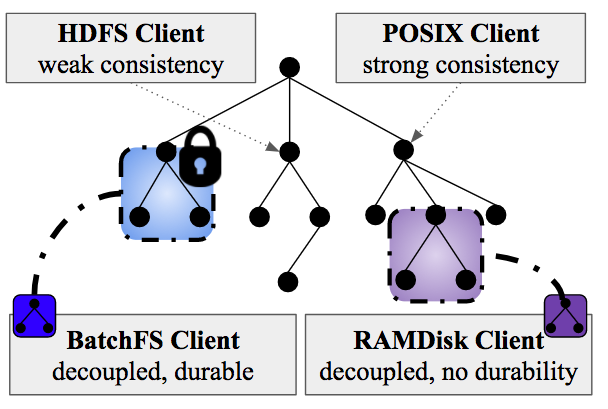
\includegraphics[width=0.35\textwidth]{figures/subtree-policies1.png}

\caption{For performance, clients can relax consistency on their subtree
({e.g.}, HDFS) or even decouple the subtree and move it locally ({e.g.},
BatchFS, RAMDisk). Decoupled subtrees can further relax durability semantics
for even better performance. Clients that require stronger guarantees ({\it
e.g.,} POSIX) can still reside in the same namespace.
}\label{fig:subtree-policies}

\end{figure}

% What is HPC doing?
To address this, developers are relaxing the consistency and durability
semantics in the file system because weaker guarantees are sufficient for their
applications. For example, many batch style jobs do not need the strong
consistency that the file system provides, so
BatchFS~\cite{zheng:pdsw2014-batchfs} and DeltaFS~\cite{zheng:pdsw2015-deltafs}
do more client-side processing and merge updates when the job is done. HPC
developers are turning to these non-POSIX solutions because their applications
are well-understood ({\it e.g.}, well-defined read/write phases,
synchronization only needed during certain phases, workflows describing
computation, etc.) and because these applications wreak havoc on file systems designed for
general-purpose workloads ({\it e.g.}, checkpoint-restart's N-N and N-1 create
patterns).

% One example
One popular approach for relaxing consistency and durability is to ``decouple
the namespace", where clients lock the subtree they want exclusive access to as
a way to tell the file system that the subtree is important or may cause
resource contention in the near-future~\cite{grider:pdsw2015-marfs,
zheng:pdsw2015-deltafs, zheng:pdsw2014-batchfs, ren:sc2014-indexfs,
bent:slides-twotiers}. Then the file system can change its internal structure
to optimize performance. For example, the file system could enter a mode that
prevents other clients from interfering with the decoupled directory.  This
delayed merge ({\it i.e.} a form of eventual consistency) and relaxed
durability improves performance and scalability by avoiding the costs of remote
procedure calls (RPCs), synchronization, false sharing, and serialization.
While the performance benefits of decoupling the namespace are obvious,
applications that rely on the file system's guarantees must be deployed on an
entirely different system or re-written to coordinate strong
consistency/durability themselves.

%\begin{table}
%\begin{tabular}{ r | l }
%  Subtree         & Example \\\hline
%  (1)   & \{Index, Batch\}FS~\cite{ren:sc2014-indexfs, zheng:pdsw2014-batchfs} \\
%  (2)   & \{Index, Ceph\}FS~\cite{ren:sc2014-indexfs, weil:sc2004-dyn-metadata} \\
%  (3)   & RAMDisk \\
%  (4)   & DeltaFS~\cite{zheng:pdsw2015-deltafs} \\
%\end{tabular}
%
%\caption{State-of-the-art systems in HPC improve file system metadata
%performance by relaxing consistency and durability guarantees. Note that
%IndexFS also supports weak consistency with bulk inserts.
%\label{table:namespaces}} \end{table}

% What did we do
To address this problem, we present an API and framework that lets developers
dynamically control the consistency and durability guarantees for subtrees in
the file system namespace.  Figure~\ref{fig:subtree-policies} shows a setup in
our proposed system where a single global namespace has subtrees for
applications optimized with techniques from different state-of-the-art HPC
architectures.  The HDFS\footnote{This is example is not directly evaluated in
this paper, although a similar use case is explored in~\S\ref{use-case-1}}
subtree has weaker consistency than strong consistency because it  does not
guarantee that all updates are not immediately seen by all servers; the BatchFS
and RAMDisk subtrees are decoupled from the global namespace and have similar
consistency/durability behavior to those systems; and the POSIX subtree retains
the rigidity of POSIX's strong consistency.

Our prototype system, Cudele, achieves this by exposing ``mechanisms" that
developers use to specify their preferred semantics.  Cudele supports 3 forms
of consistency (invisible, weak, and strong) and 3 degrees of durability (none,
local, and global) giving the user a wide range of policies and optimizations
that can be custom fit to an application. We make the following contributions:

\begin{enumerate}

  \item a prototype that lets developers choose from a range of
  consistency and durability semantics (9 permutations), allowing them to dynamically custom
  fit the storage system to the application.

  \item an API for selecting consistency/durability policies and assigning
  them to subtrees in the file system namespace.

  \item an apples-to-apples comparison of the strategies used in recently proposed research systems against
  previously unexplored metadata designs, all implemented using Cudele.

\end{enumerate}

% Results
Our results confirm the assertions of ``clean-state" research systems that
decouple namespaces; specifically that the technique drastically improves
performance (104\(\times\) speed up) but we go a step further by quantifying
the costs of merging updates (7\(\times\) slow down) and maintaining durability
(\(10\times\) slow down). We also show the effect of having a metadata specific
file format in systems that are based on in-memory data structures.  We scale
up to 20 clients executing an extremely metadata intensive job because this
workload exhausts the resources of a single metadata server for the code base we
built on.  Partitioning and replicating metadata across a cluster can be
controlled with something like Mantle~\cite{sevilla:sc15-mantle}, but in this
paper we show the capacity and performance of a metadata server with superior
metadata protocols, which should be used to inform load balancing decisions.

In the remainder of the paper, Section~\ref{sec:posix-overheads} quantifies the
cost of POSIX consistency and system-defined durability and
Section~\ref{sec:methodology-decoupled-namespaces} presents the Cudele
prototype and API. Section~\ref{sec:implementation} describes the Cudele
mechanisms and shows how re-using internal subsystems results in an
implementation of less than 500 lines of code. The evaluation in
Section~\ref{sec:evaluation} quantifies the overheads and performance gains of
explored and previously unexplored metadata designs.
Section~\ref{sec:related-work} places Cudele in the context of other related
work.


\section{POSIX IO Overheads}
\label{sec:posix-overheads}

\begin{figure}[tb]
\centering
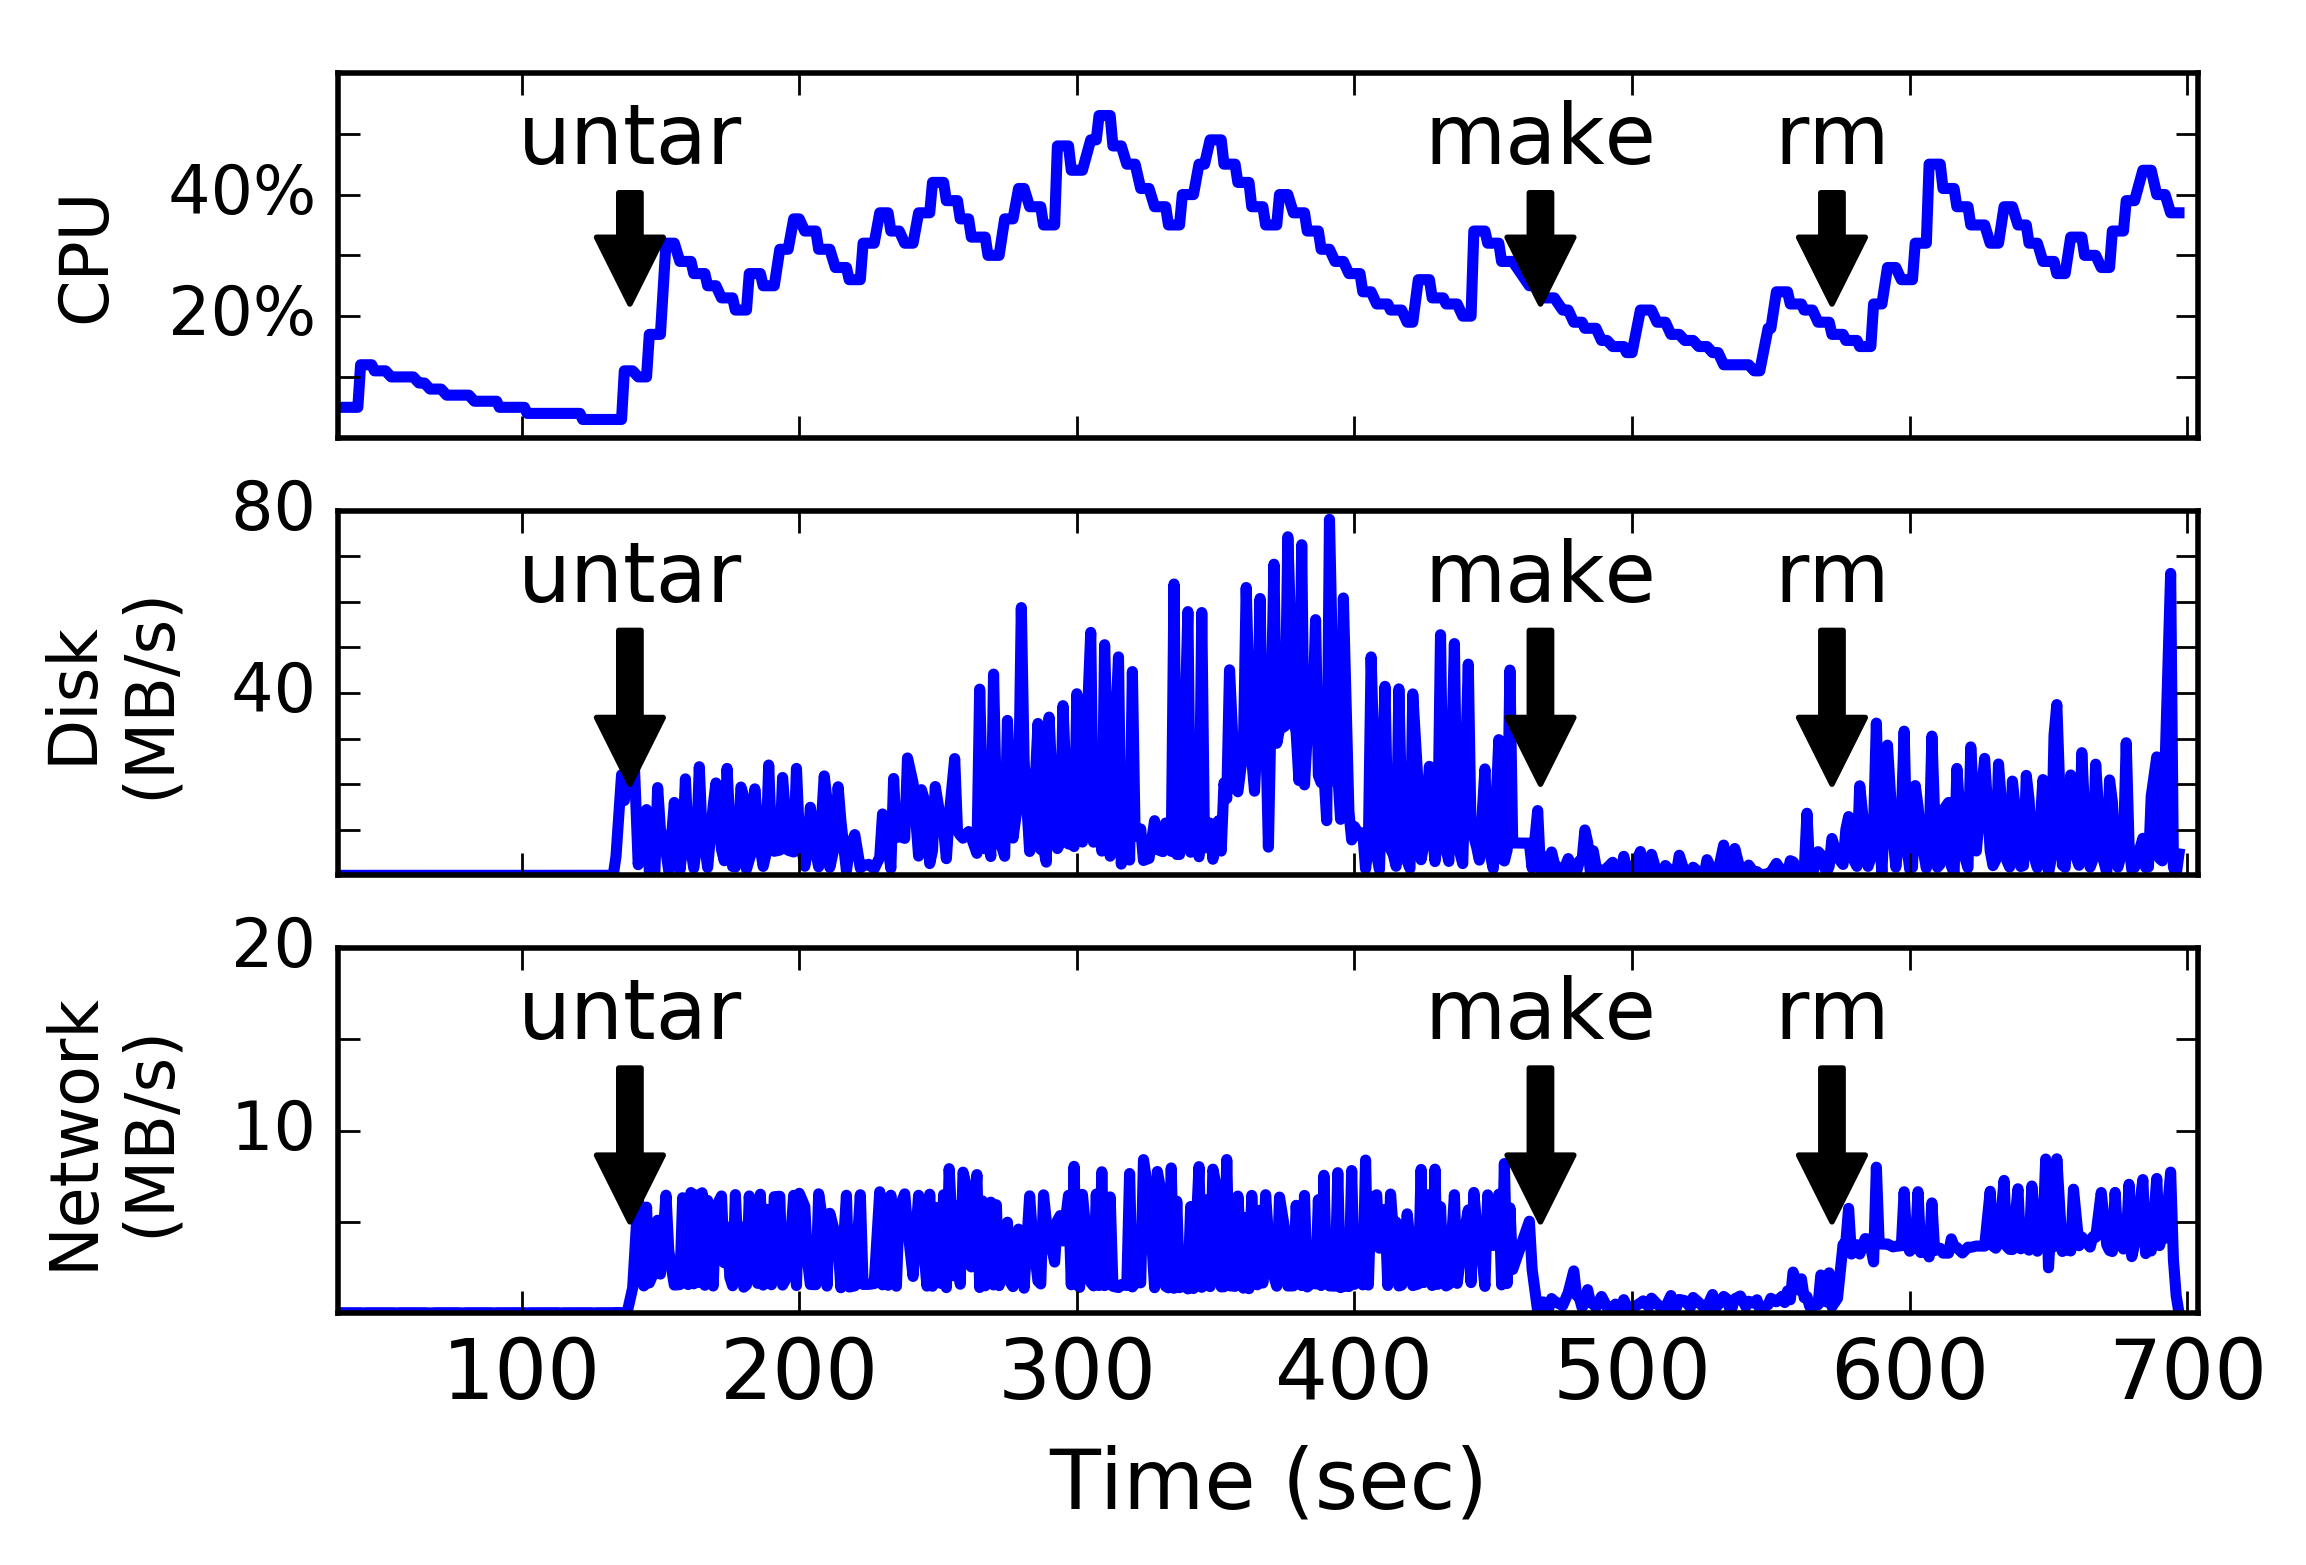
\includegraphics[width=1\linewidth]{./graphs/overhead-creates.png}
\caption{Create-heavy workloads (such as \texttt{untar}) incur the highest disk, network, and
CPU utilization because of the consistency and durability demands of
CephFS.}\label{fig:overhead-creates}
\end{figure}

In our examination of the overheads of POSIX IO we benchmark and analyze
CephFS, the file system that uses Ceph's object store ({\it i.e.} RADOS) to
store its data and metadata. To show how the file system behaves under high
metadata load we use a create-heavy workload.  During this process we
discovered, based on the analysis and breakdown of costs, that durability and
consistency have high overhead but we urge the reader to keep in mind that this
file system is an implementation of one set of design decisions and our goal
here is to highlight the effect that those decisions have on performance.

Figure~\ref{fig:overhead-creates} shows the resource utilization of compiling
the Linux kernel.  The \texttt{untar} phase, which is characterized by many
creates, has the highest resource usage (combined CPU, network, and disk)
because of the number of RPCs needed for consistency and durability. The RPCs
are also serialized because the metadata server is single threaded; although
na\"{\i}ve, this design is common because of the complexity of multi-threaded
metadata servers~\cite{konstantinos:pdsw2014-lustre-metadata}.  Traditional
file system techniques for improving performance, such as caching inodes, do
not help for create-heavy workloads.  In this section, we quantify the costs of
consistency and durability in CephFS.  At the end of each subsection we compare
the approach to ``decoupled namespaces", the technique in related work that
detaches subtrees from the global namespace to relax consistency/durability
guarantees. 

\subsection{Durability}
\label{sec:durability}

\begin{figure*}[t]
  \centering
  \begin{subfigure}[b]{.3\linewidth}
      \centering
      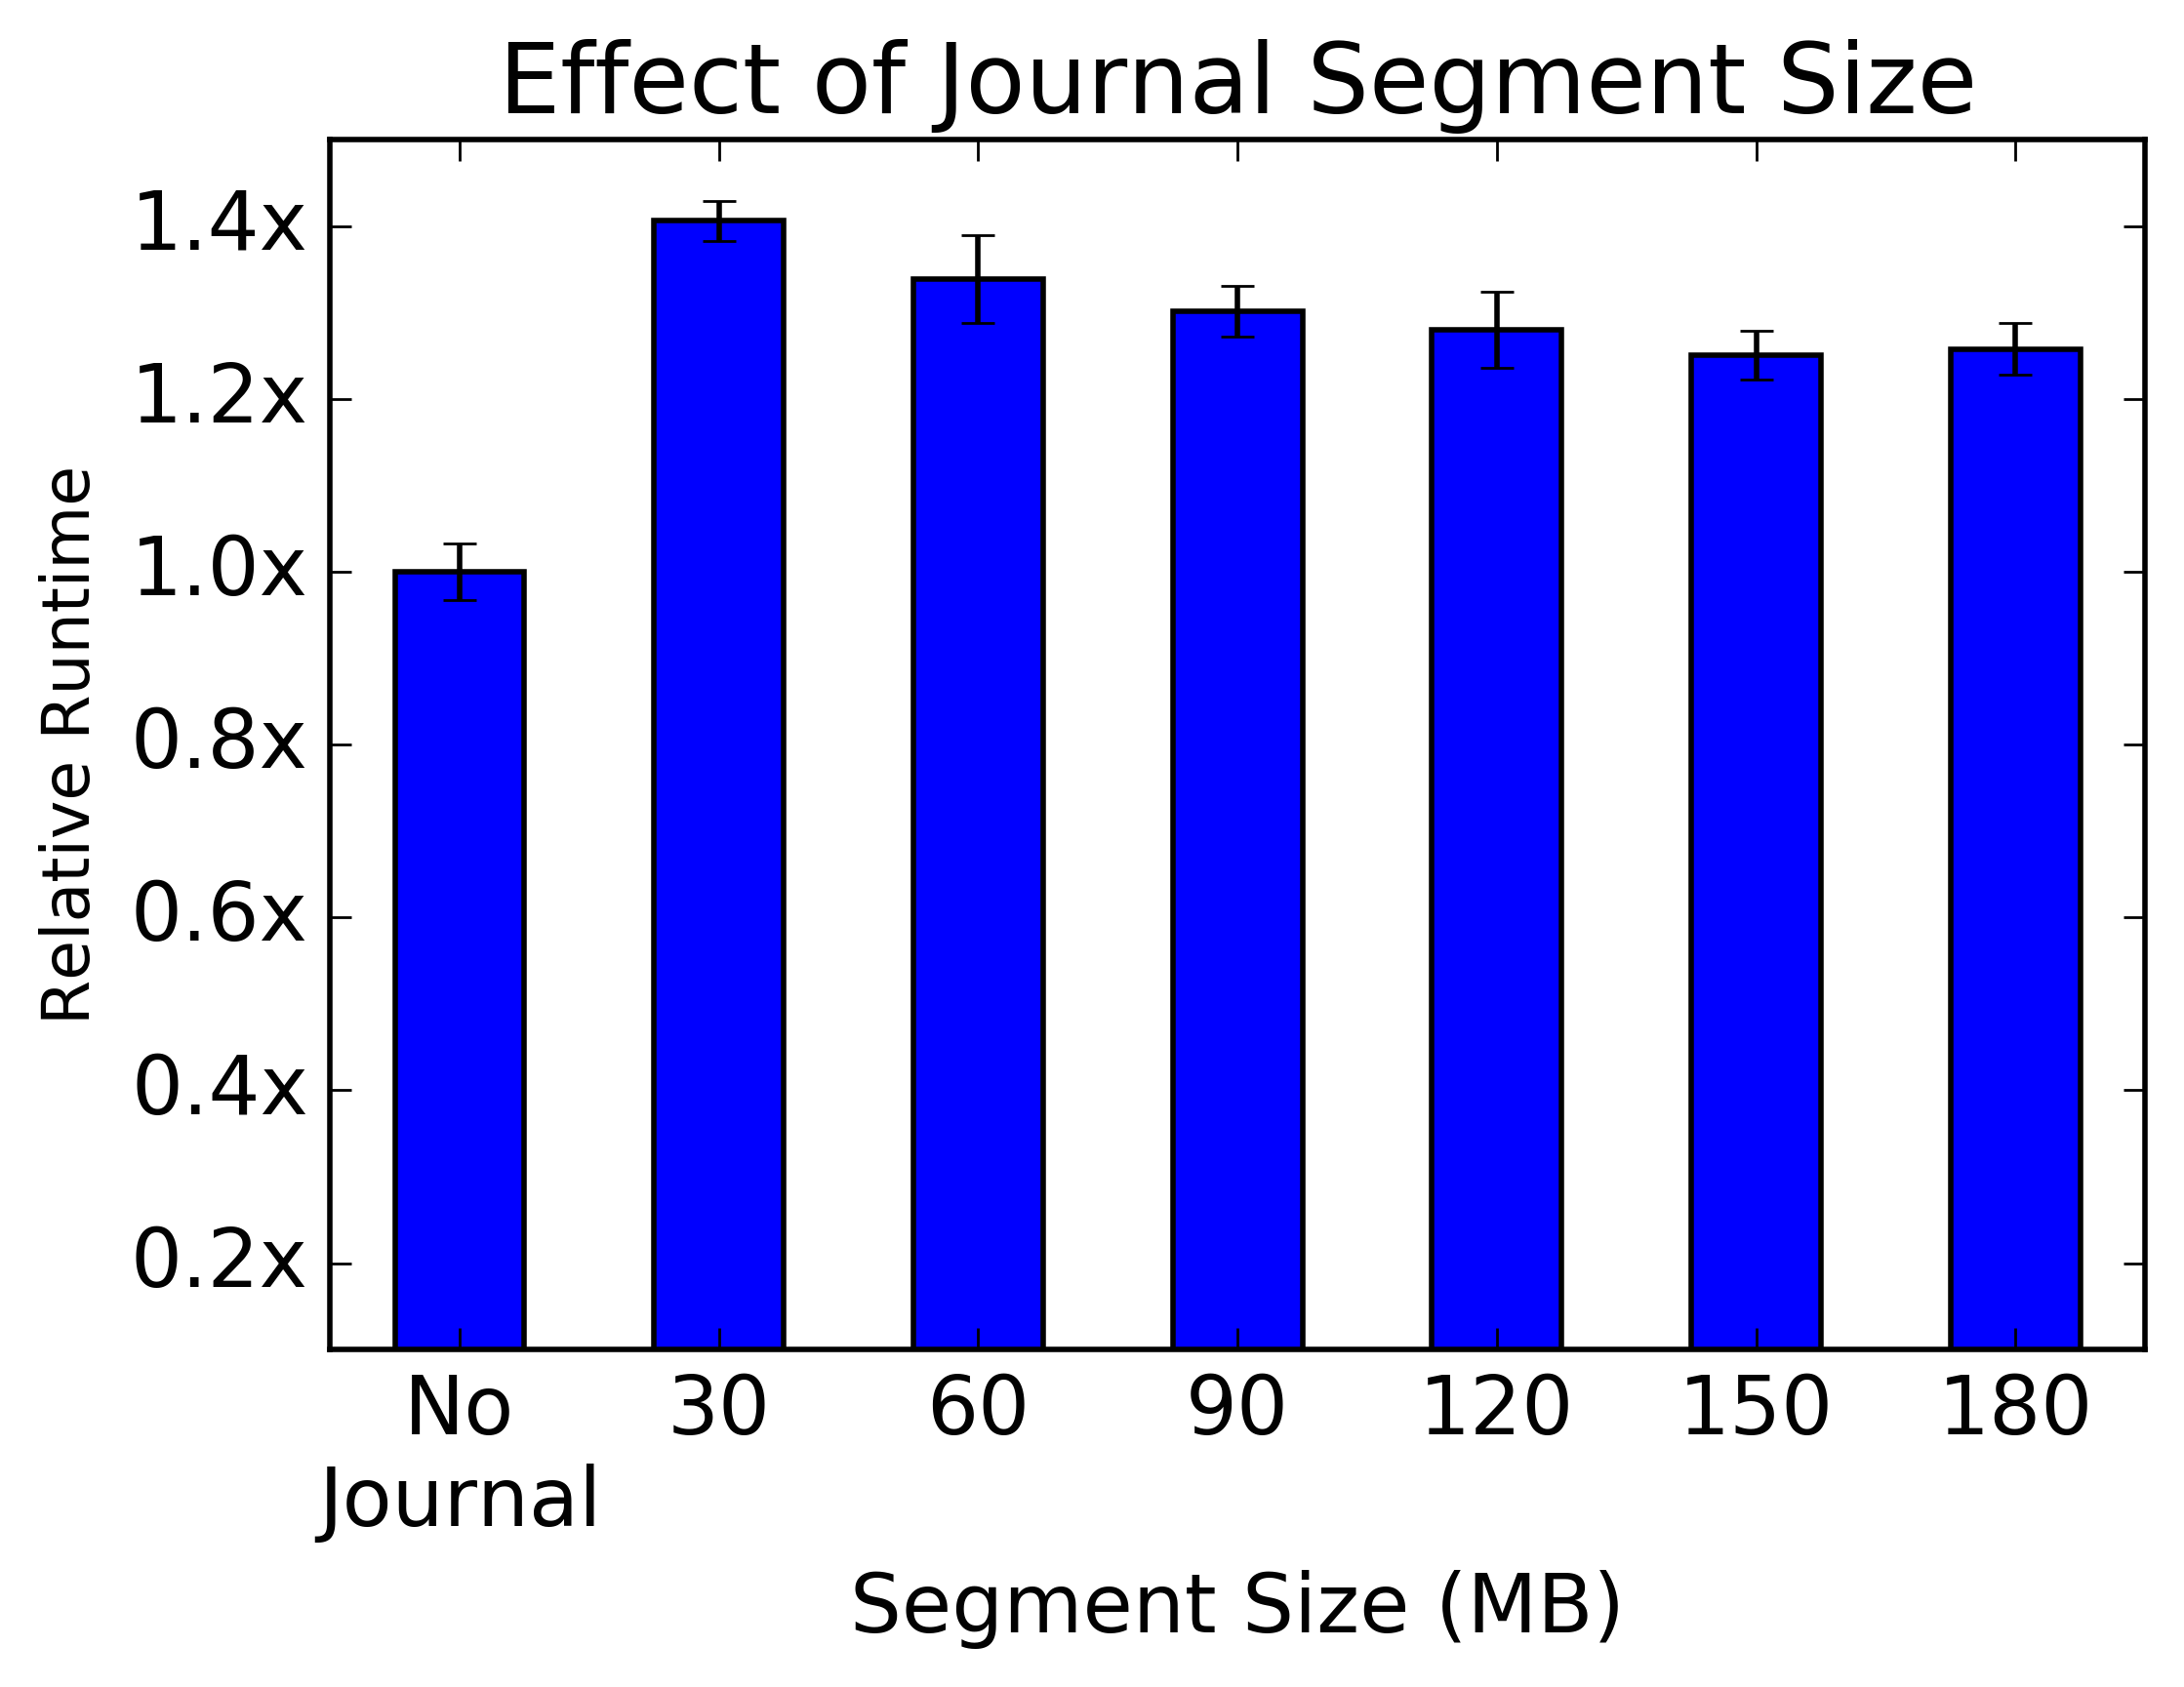
\includegraphics[width=1.0\linewidth]{graphs/slowdown-journal.png}
      \caption{Runtime normalized to no journal} \label{fig:overhead-a}
  \end{subfigure}
  \begin{subfigure}[b]{.3\linewidth}
      \centering
      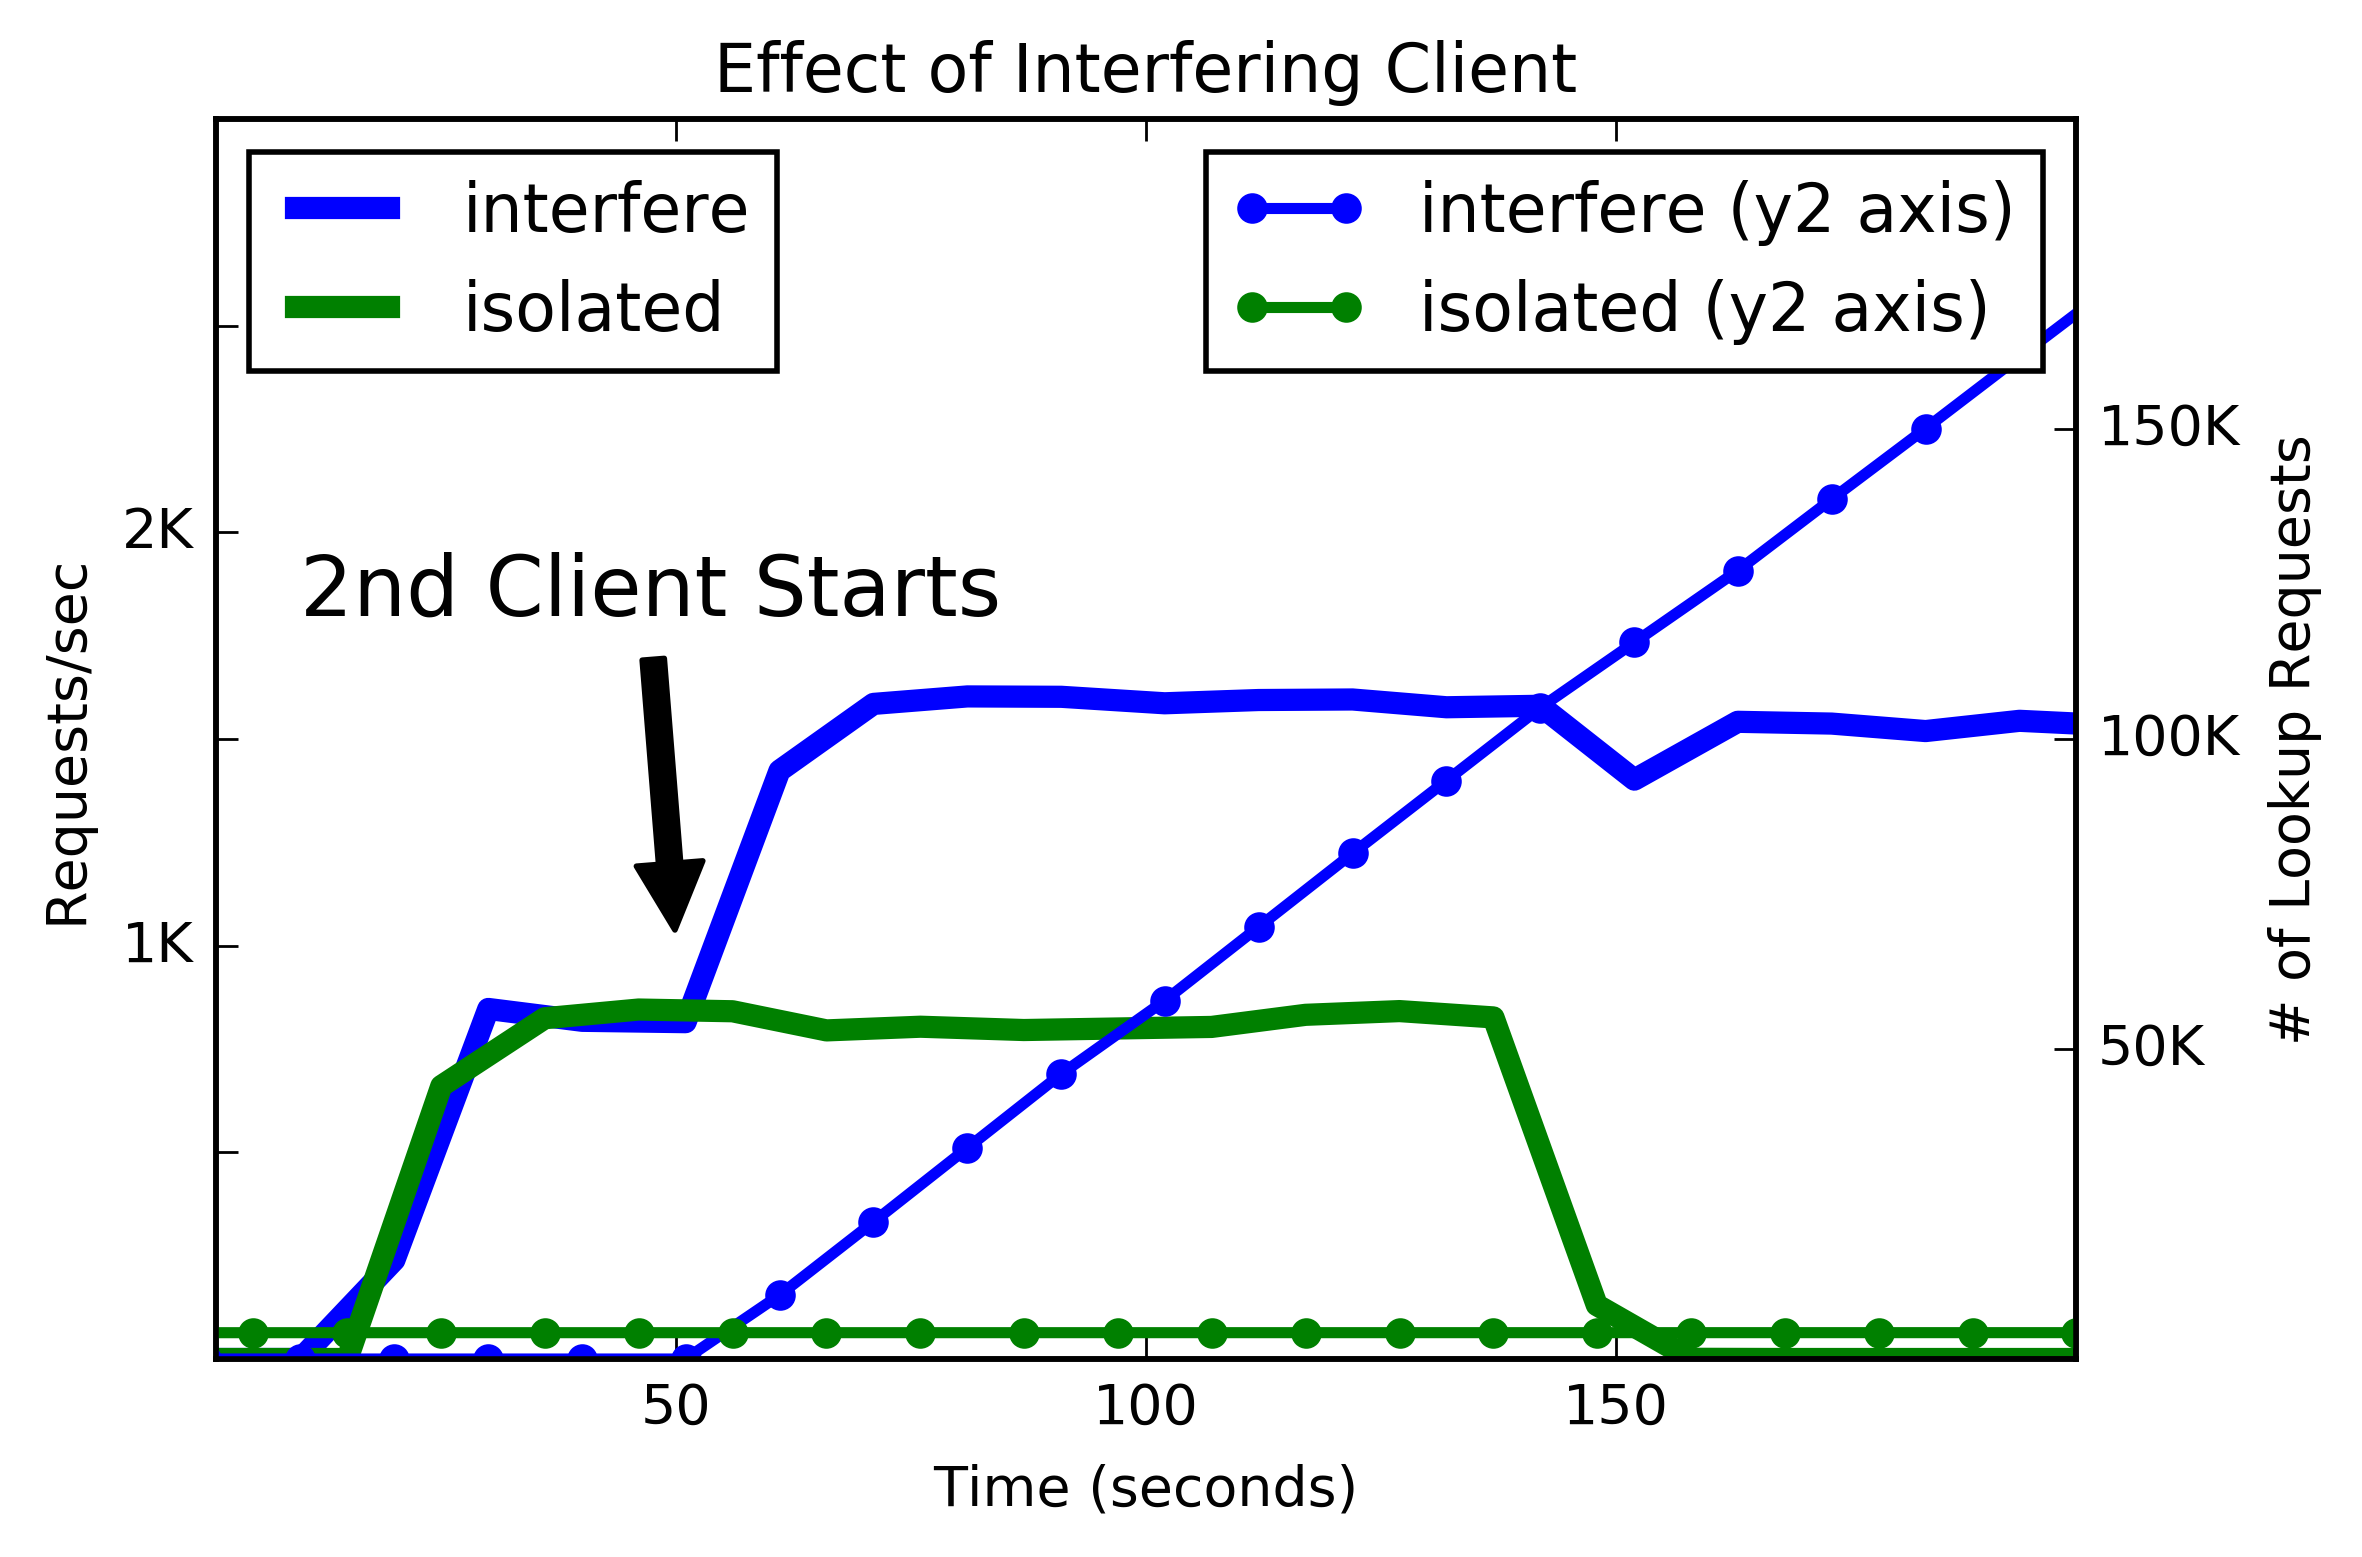
\includegraphics[width=1.2\linewidth]{graphs/behavior-interfere.png}
      \caption{Interference forces \texttt{lookup()}s}
      \label{fig:overhead-b}
  \end{subfigure}
  \begin{subfigure}[b]{.3\linewidth}
      \centering
      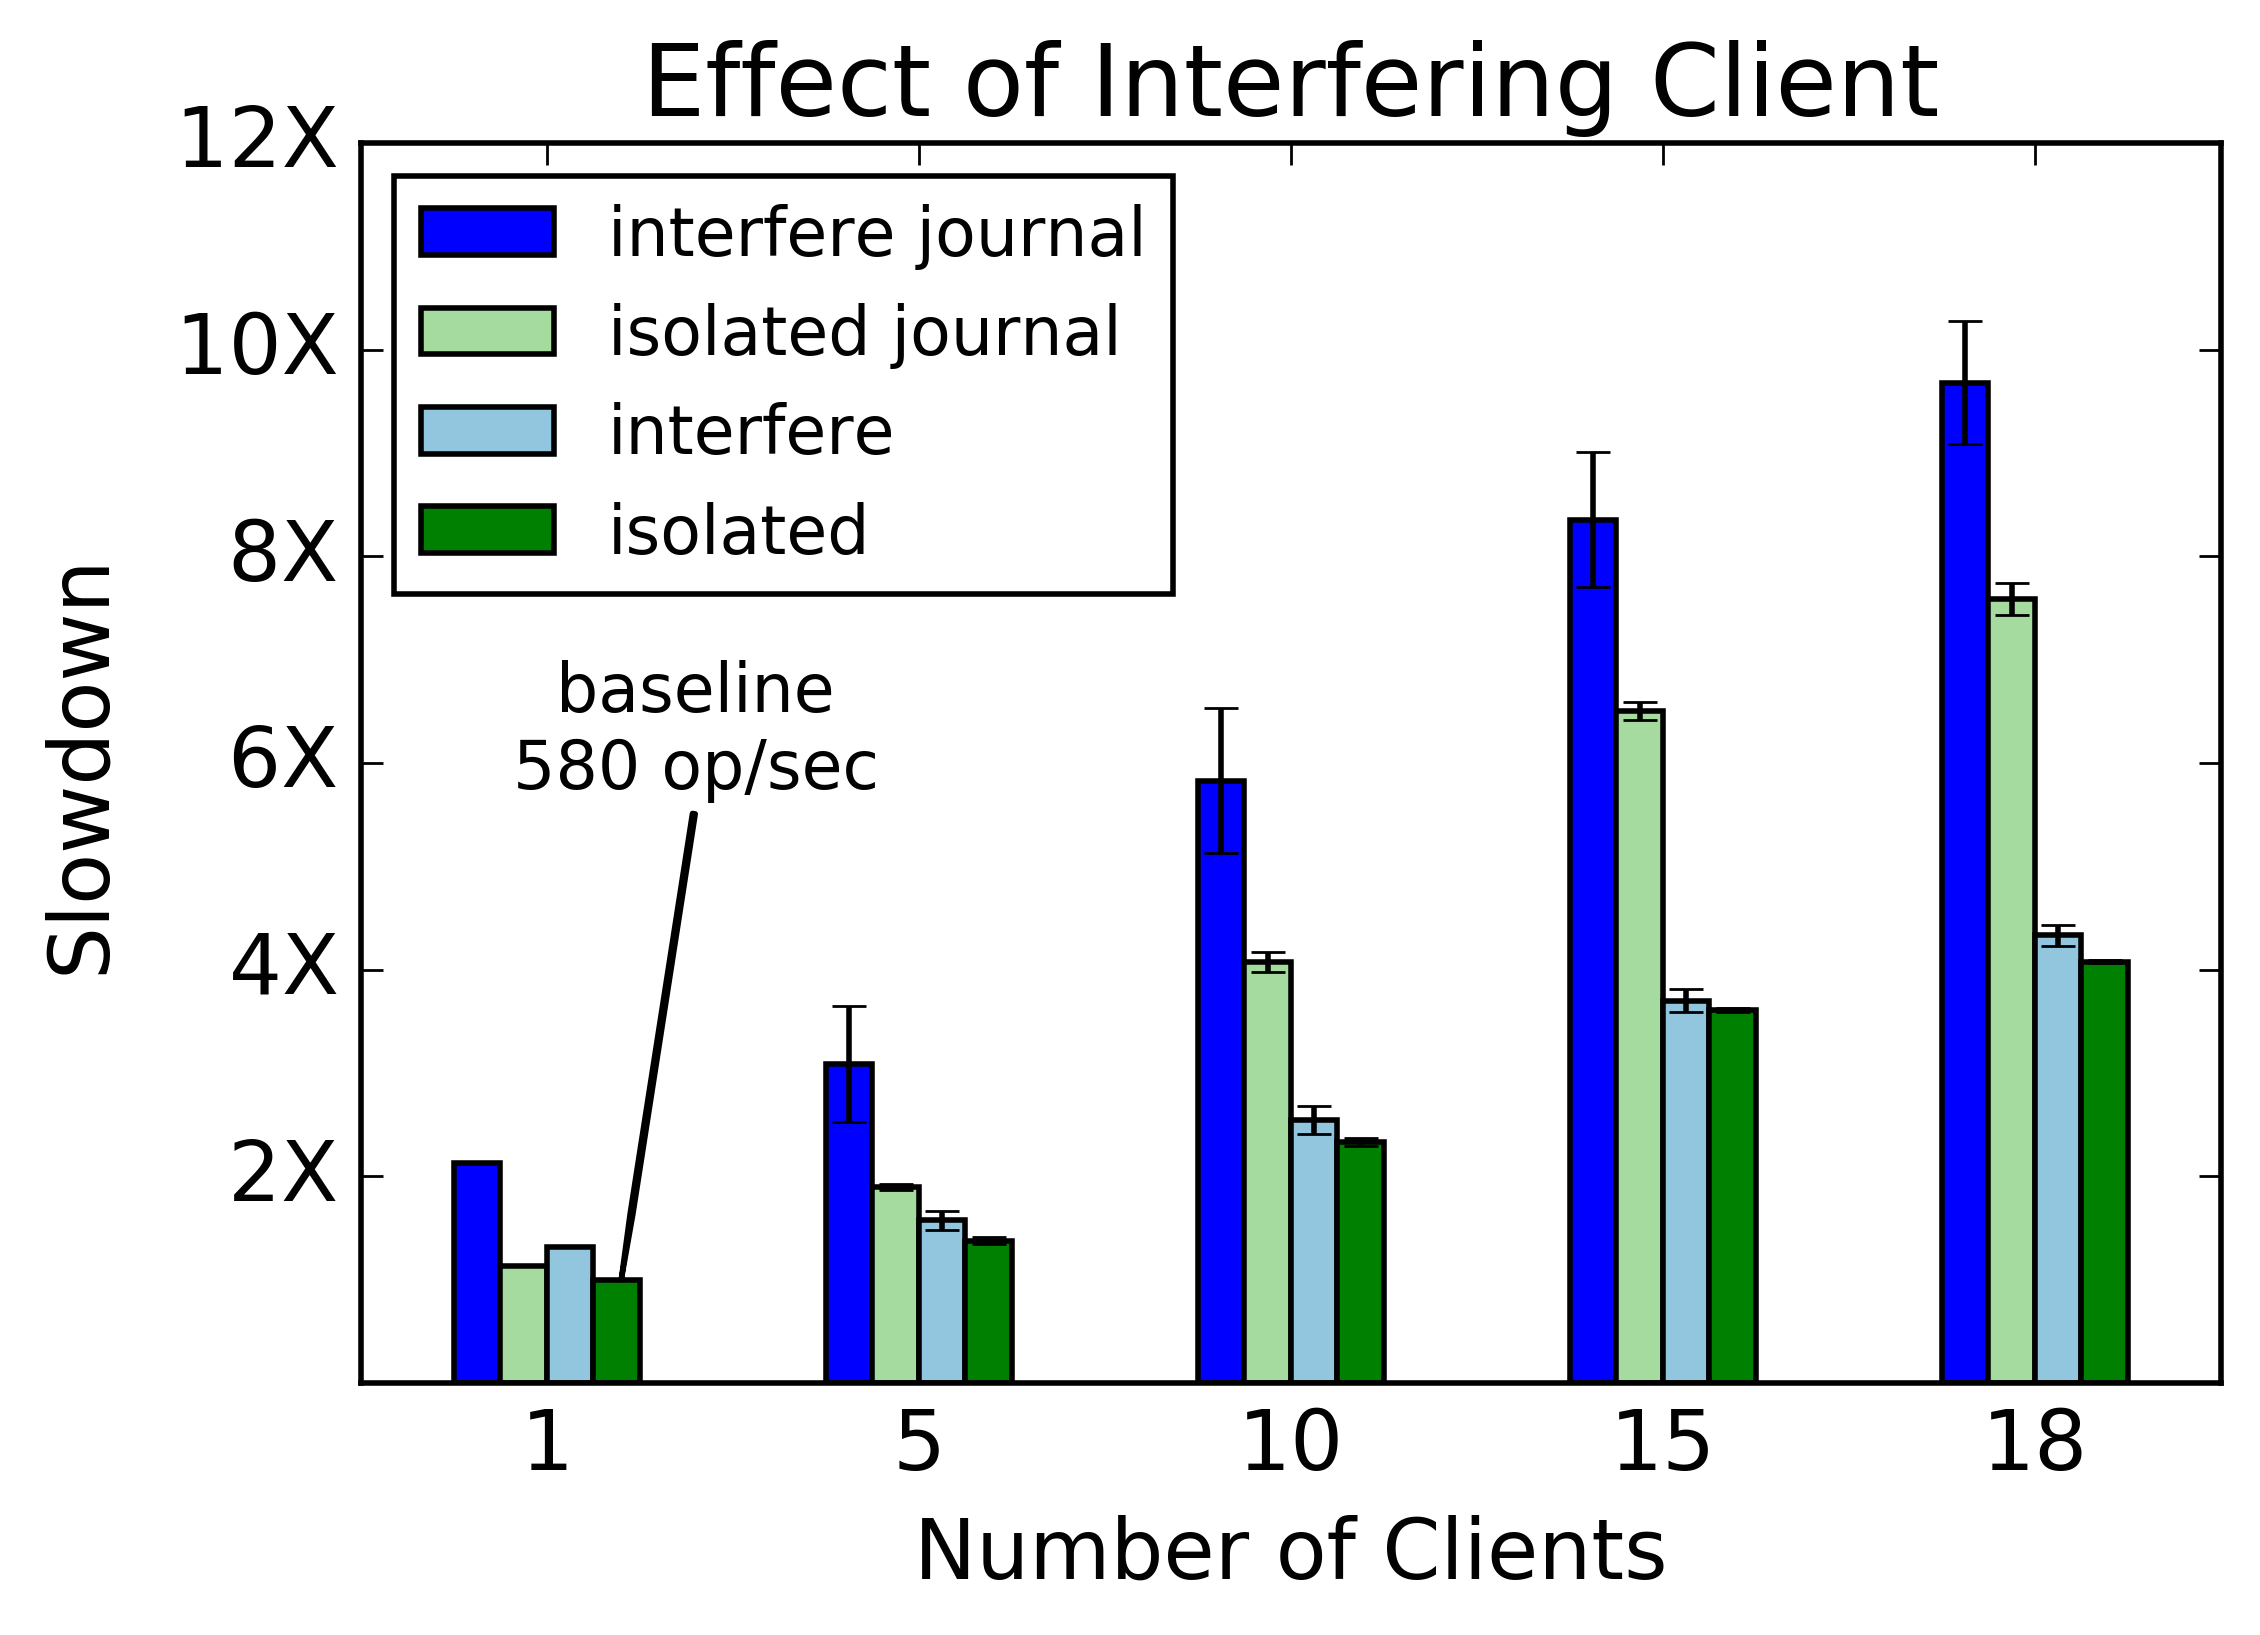
\includegraphics[width=1.0\linewidth]{graphs/slowdown-interfere-scale.png}
      \caption{Interference hurts variability}
      \label{fig:overhead-c}
  \end{subfigure}
  \caption{The overhead of durability and strong consistency in CephFS.
  (a) shows the effect of different journal segment sizes, which are streamed
  into the object store for fault tolerance. (b) and (c) show that when a second
  client ``interferes", capabilities are revoked and metadata servers do more
  work.  \label{fig:overhead}}
\end{figure*}

% what is durability
While durability is not specified by POSIX IO, users expect that files they
create or modify survive failures.  We define three types of durability:
global, local, and none.  Global durability means that the client or server can
fail at any time and metadata will not be lost because it is ``safe" ({\it
i.e.} striped or replicated across a cluster). Local durability means that
metadata can be lost if the client or server stays down after a failure. None
means that metadata is volatile and that the system provides no guarantees when
clients or servers fail.  None is different than local durability because
regardless of the type failure, metadata will be lost when components die in a
None configuration.

% - sequential IO, trim redundant operations
\textbf{CephFS Design}: A journal of metadata updates that streams into the
resilient object store. Similar to LFS~\cite{rosenblum:acm1992-LFS} and
WAFL~\cite{hitz:wtec1994-WAFL} the metadata journal is designed to be large
(on the order of MBs) which ensures (1) sequential writes into the object store
and (2) the ability for daemons to trim redundant or irrelevant journal
entries.  The journal is striped over objects where multiple journal updates
can reside on the same object. There are two tunables for controlling the
journal: the segment size and the number of segments that can be written in
parallel. Unless the journal saturates memory or CPU resources, larger values
for these tunables results in better performance.

% purpose of the journal
In addition to the metadata journal, CephFS also represents metadata in RADOS
as a metadata store, where directories and their file inodes are stored as
objects.  The metadata server applies the updates in the journal to the
metadata store when the journal reaches a certain size. The metadata store is
optimized for recovery ({\it i.e.} reading) while the metadata journal is
write-optimized.

%\begin{figure}[tb] \centering
%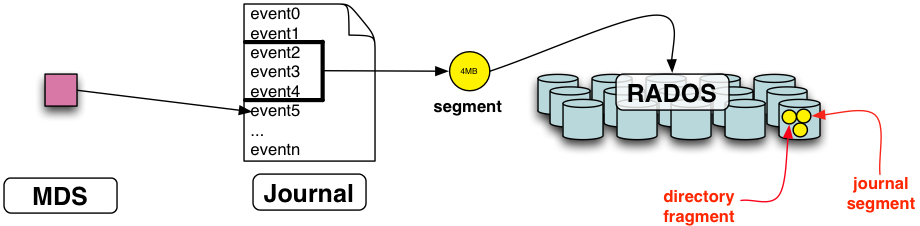
\includegraphics[width=1\linewidth]{./figures/journal.png} 
%\caption{CephFS has two views of the file system namespace: a journal of
%metadata updates and a metadata store. For fault tolerance, they are stored in
%the object store as segments and fragments, respectively.
%\label{fig:journal}}
%\end{figure}

% Effects on performance
Figure~\ref{fig:overhead-a} shows the
effect of journaling of different journal segment sizes; the larger the segment
size the bigger that the writes into the object store are. The trade-off for
better performance is memory consumption because larger segments take up
more space for buffering. When journaling is on, 
the metadata server periodically stops serving requests to flush ({\it i.e.}
apply journal updates) to the metadata store.  The journal overhead is
sufficient enough to slow down metadata throughput but not so much as to
overwhelm the bandwidth of the object store. We measured our peak bandwidth to
be 100MB/s, which is the speed of our network link.

\textbf{Comparison to decoupled namespaces}: In BatchFS and DeltaFS, to the
best of our knowledge, when a client or server fails there is no recovery
scheme. For BatchFS, if a client fails when it is writing to the local
log-structured merged tree (implemented as an
SSTable~\cite{ren:atc2013-tablefs}) then those batched metadata operations are
lost. For DeltaFS, if the client fails then, on restart, the computation does
the work again -- since the snapshots of the namespace are never globally
consistent and there is no ground truth.  On the server side, BatchFS and
DeltaFS use IndexFS. IndexFS writes metadata to SSTables, which initially
reside in memory but are later flushed to the underlying distributed file
system.

\subsection{Strong Consistency}
\label{sec:strong-consistency}

Access to metadata in a POSIX IO-compliant file system is strongly consistent, so
reads and writes to the same inode or directory are globally ordered.  The
synchronization and serialization machinery needed to ensure that all clients
see the same state has high overhead.

\textbf{CephFS Design}: Capabilities keep metadata strongly
consistent. To reduce the number of RPCs needed for consistency, clients can
obtain capabilities for reading, creating and updating inodes, as well as caching reads,
buffering writes, changing the file size, and performing lazy IO.

% inode cache - reduces RPCs (lookups for create, readdirs for stats)
To keep track of the read caching and write buffering capabilities, the clients
and metadata servers agree on the state of each inode using an inode cache.  If
a client has the directory inode cached it can do metadata writes ({\it e.g.},
create) with a single RPC. If the client is not caching the directory inode
then it must do an extra RPC to determine if the file exists.  Unless the
client immediately reads all the inodes in the cache ({\it i.e.} \texttt{ls
-alR}), the inode cache is less useful for create-heavy workloads.

% benefits PROBLEM -- IS THIS THE METADATA PROTOCOL OR JUST THE OVERLOADEDNESS?
The benefits of caching the directory inode when creating files is shown in
Figure~\ref{fig:overhead-b}. The colors show the behavior of the client for two
different runs.  If only one client is creating files in a directory
(``isolated" curve on \(y1\) axis) then that client can lookup the existence of
new files locally before issuing a create request to the metadata server. If
another client starts creating files in the same directory (``interfere" curve
on \(y1\) axis) then the directory inode transitions out of read caching and
the first client must send \texttt{lookup()}s to the metadata server
(``interfere" curve on \(y2\) axis). These extra requests increase the
throughput of the ``interfere" curve because the metadata server can handle the
extra load but performance suffers.  This degradation is shown in
Figure~\ref{fig:overhead-c}, where we scale the number of clients and show the
slowdown of the slowest client.  The results are normalized to a single
isolated client without a metadata server journal.  For the ``interfere" bars,
each client creates files in private directories and at 30 seconds we launch
another process that creates files in those directories. 18 clients is the
maximum number the metadata server could handle for this metadata-intensive
workload; at higher client load, the metadata server started complaining about
laggy and unresponsive requests.

% TODO: what is the cost of trimming the cache?
% TODO: does CephFS still cache inodes when I turn off caching? Why is still keeping inodes in memory? Gah!

\textbf{Comparison to decoupled namespaces}: Decoupled namespaces
merge batches of metadata operations into the global namespaces when the job
completes.  In BatchFS the merge is delayed by the application using an API to
switch between asynchronous to synchronous mode. The merge itself is explicitly
managed by the application but future work looks at more automated
methodologies. In DeltaFS snapshots of the metadata subtrees stays on the client
machines; there is no ground truth and consistent namespaces are constructed
and resolved at application read time or when a 3rd party system ({\it e.g.},
middleware, scheduler, etc.) needs a view of the metadata. As a result, all the
overheads of maintaining consistency that we showed above are delayed until the
merge phase.

\section{Methodology: Global Namespace with Per-Subtree Consistency/Durability}
\label{sec:methodology-decoupled-namespaces}

\begin{figure}[tb]
\centering
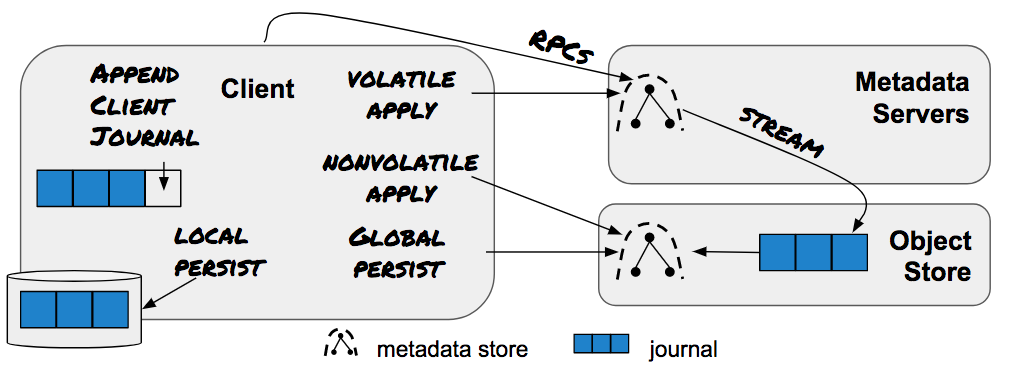
\includegraphics[width=90mm]{figures/fig-decouple.png}
\caption{Applications decouple the namespace, write updates to a local journal,
and delay metadata updates using the CudeleFS Mechanisms }\label{fig:decouple}
\end{figure}

\begin{table}
\begin{tabular}{ r | l }
  Mechanism         & Description \\\hline
  RPCs              & round trip remote procedure calls \\
  Stream            & stream journal into object store \\
  Append Client Journal & events appended to in-memory journal \\
  Volatile Apply    & apply to metadata store in obj store \\
  Nonvolatile Apply & apply to metadata store in memory \\
  Local Persist     & journal saved to client's disk \\
  Global Persist    & journal saved in object store \\
\end{tabular}
\caption{The CudeleFS mechanisms are composed together to form consistency and
durability semantics.\label{table:mechanisms}} 
\end{table}

In this section we describe CudeleFS, our file system that lets users
assign consistency and durability semantics to subtrees in the global
namespace. A \textbf{mechanism} is an abstraction and basic building block for
constructing consistency and durability guarantees. CudeleFS exposes these
mechanisms and the user composes them together to construct
\textbf{policies}. These policies are assigned to subtrees and they dictate how
the file system should handle operations within that subtree.  Below, we
describe the mechanisms, the policies, and the API for assigning policies to
subtrees.

\subsection{The CudeleFS Mechanisms}
\label{sec:the-cudelesfs-mechanisms}

% describe the figure
Figure~\ref{fig:decouple} shows the mechanisms (labeled arrows) in CudeleFS and
which daemon(s) they are performed by.  Table~\ref{table:mechanisms} has a
description of what each mechanism does.  Decoupled clients use the ``Append Client Journal"
mechanism to append metadata updates to a local, in-memory journal. Once the
job is complete, the system calls CudeleFS mechanisms to achieve the desired
consistency/durability semantics.  CudeleFS provides a library for clients to
link into and all operations are performed by the client.  

\subsubsection{Mechanisms Used for Consistency} ``RPCs" send remote procedure
calls for every metadata operation from the client to the metadata server,
assuming the request cannot be satisfied by the inode cache. This mechanism is
part of the default CephFS implementation and is the strongest form of
consistency because clients see metadata updates right away.  ``Nonvolatile
Apply" replays the client's journal onto the metadata cluster's metadata store.
The client's in-memory journal is written into the object store and the
metadata servers are restarted. When the metadata servers re-initialize, they
notice new journal updates in the object store and replay the events onto their
in-memory metadata stores.  ``Volatile Apply" takes the client's in-memory journal on the
client and applies the updates directly to the in-memory metadata store maintained
by the metadata servers. We say volatile because -- in exchange for peak
performance -- CudeleFS makes no consistency or durability guarantees while
``Volatile Apply" is executing.  If a concurrent update from a client occurs
there is no rule for resolving conflicts and if the client or metadata server
crashes there may be no way to recover.

% difference between apply and volatile apply
The biggest difference between ``Volatile Apply" and ``Nonvolatile Apply" is
the medium they use to communicate. ``Volatile Apply" applies updates directly
to the metadata servers' metadata store while ``Nonvolatile Apply" uses the
object store to communicate the journal of updates from the client to the
metadata servers.  ``Nonvolatile Apply" is safer but has a large performance
overhead because objects in the metadata store need to be read from and written
back to the object store.

%The metadata store and journal
%are different ways of representing the namespace.  CudeleFS presents 6
%mechanisms: RPCs, Stream, Create, Volatile Apply, Local Persist, and Global
%Persist. ``RPCs" does round trip remote procedure calls to establish
%consistency; it is the default implementation for complying with POSIX in
%CephFS. ``Stream" has the metadata servers stream a journal of metadata updates
%into the object store. ``Append Client Journal" allows clients to append metadata events to an
%in-memory journal. ``Volatile apply" 
% ``Local Persist" takes the in-memory journal and writes it to the
%client's disk. ``Global Persist" saves the journal as a an object in the object
%store from the client.  Next, we discuss how these mechanisms can be composed
%to get different consistency and durability semantics. 

\subsubsection{Mechanisms Used for Durability} ``Stream" is one of the
mechanisms used by default in CephFS.  Using existing configuration settings in
Ceph we can turn ``Stream" on and off.  If it is off, then the metadata servers
will not save journals in the object store. For ``Local Persist", clients write
serialized log events to a file on local disk and for ``Global Persist",
clients push the journal into the objects store. The overheads for both ``Local
Persist" and ``Global Persist" is the write bandwidth of the local disk and
object store, respectively.  These persist mechanisms are part of the library that
links into the client.

\subsection{Defining Policies in CudeleFS}
\label{sec:setting-policies-with-cudele}

\begin{table}[t]
\begin{center}
\begin{tabular}{ l | l | l | l }
  C \(\rightarrow\) &&& \\  
  D \(\downarrow\)  	     & invisible         & weak        & strong  \\\hline
  none                       & append client journal            & append client journal          & RPCs    \\
                             &                   & +volatile apply &         \\\hdashline
  local                      & append client journal            & append client journal          & RPCs    \\
                             & +local persist    & +local persist  & +local  \\
                             &                   & +volatile apply &  persist\\\hdashline
  global                     & append client journal            & append client journal          & RPCs    \\
                             & +global persist   & +global persist & +stream \\
                             &                   & +volatile apply &         \\
\end{tabular}

\caption{Users can explore the consistency (C) and
durability (D) spectrums by composing CudeleFS mechanisms. 
\label{table:spectrum}}
\end{center}
\end{table}



% describe table
The spectrum of consistency and durability guarantees that users can
construct is shown in Table~\ref{table:spectrum}. The columns are the different
consistency semantics and the rows cover the spectrum of durability guarantees.
For consistency: ``invisible" means the system does not handle merging updates
into a global namespace and it is assumed that middleware or the application
manages consistency lazily; ``weak" merges updates at some time in the
future ({\it e.g.}, when the system has time, when the number of updates reaches a
certain threshold, when the client is done writing, etc.); and updates in
``strong" consistency are seen immediately by all clients. For durability,
``none" means that updates are volatile and will be lost on a failure. Stronger
guarantees are made with ``local", which means updates will be retained if the
client node recovers, and ``global", where all updates are always recoverable.

% which system they represent and which are impossible
Existing, state-of-the-art systems in HPC can be represented by the cells in
Table~\ref{table:spectrum}.  POSIX-compliant systems like CephFS and IndexFS
have global consistency and durability ~\footnote{This is the normal case.
IndexFS also has bulk merge which would transition the system into ``weak
consistency"}; DeltaFS uses ``invisible" consistency and ``local" durability
and BatchFS uses ``weak" consistency and ``local" durability. These systems
have other features that could push them into different semantics but we assign
labels here based on the points emphasized in the papers.  To compose the
mechanisms users inject which mechanisms to run and which to use in parallel
using a domain specific language.  Although we can achieve all permutations of
the different guarantees in Table~\ref{table:spectrum}, not all of them make
sense. For example, it makes little sense to do \texttt{append client journal+RPCs} since
both mechanisms do the same thing or \texttt{stream+save} since ``global"
durability is stronger and has more overhead than ``local" durability. 

% talk of eventual consistency
The consistency and durability properties in Table~\ref{table:spectrum} are not
guaranteed until all mechanisms in the cell are complete. The compositions
should be considered atomic and there are no guarantees while transitioning
between policies. For example, updates are not deemed to have ``global" durability until
they are safely saved in the object store. If a failure occurs during ``global
persist" or if we inject a new policy that changes a subtree from ``local
persist" to ``global persist", CudeleFS makes no guarantee until the mechanisms are
complete.

\subsection{CudeleFS Namespace API}
\label{sec:cudelefs-namespace-api}



% the interface
Users control consistency and durability for subtrees by contacting the monitor
daemon with a directory path and presenting a policies configuration file.
For example, (msevilla/mydir, policies.yml) would decouple the path
``msevilla/mydir" and would apply the policies in ``policies.yml".  The
policies file supports the following parameters (default values are in parenthesis):

\begin{itemize}

  \item \texttt{consistency}: which consistency model to use (\texttt{RPCs})

  \item \texttt{durability}: which durability model to use (\texttt{stream})

  \item \texttt{allocated\_inodes}: the number of inodes to provision to the
  decoupled namespace (100)

  \item \texttt{interfere\_policy}: how to handle a request from another
  client targeted at this subtree (\texttt{allow}))

\end{itemize}

The ``Consistency" and ``Durability" parameters are set to the CudeleFS
mechanisms; they can be composed (\(+\)) or run in parallel (\(|\|\)).
``Allocated Inodes" is a way for the application to specify how many files it
intends to create. It is a contract so that the file system can provision
enough resources for the incumbent merge and so it can give valid inodes to
other clients. The inodes can be used anywhere within the decoupled namespace
({i.e.} at any depth in the subtree).

% description
``Interfere Policy" has two settings: \texttt{block} and \texttt{allow}.
For \texttt{block}, any requests to this part of the namespace returns with
``Device is busy", which will spare the metadata server from wasting resources
for updates that may get overwritten. If the application does not mind losing
updates, for example it wants approximations for results that take too long to
compute, it can select \texttt{allow}. In this case, metadata from the interfering client will be
written and the computation from the decoupled namespace will take priority at
merge time because the results are more accurate.

% examples
Given these default values decoupling the namespace with an empty policies file
would give the application 100 inodes but the subtree would behave like the
existing CephFS implementation. To implement DeltaFS on CudeleFS, the user
would use the configuration:

\begin{listing}[h]
\begin{minted}[xleftmargin=21pt,fontsize=\footnotesize,
               tabsize=4]{js}
{     
    "allocated_inodes": "100000"
    "interfere_policy": "block"
    "consistency": "append_client_journal"
    "durability": "local_persist"
}
\end{minted}
\end{listing}

BatchFS merges updates into the global namespace after the job is complete.
This can be achieved with by composing two mechanisms: 

\begin{listing}[h]
\begin{minted}[xleftmargin=21pt,fontsize=\footnotesize,
               tabsize=4]{js}
{     
  "allocated_inodes": "100000"
  "interfere_policy": "block"
  "consistency": "append_client_journal+volatile_apply"
  "durability": "local_persist"
}
\end{minted}
\end{listing}

\section{Implementation}
\label{sec:implementation}

We use a programmable storage approach~\cite{sevilla:eurosys17} to design
Cudele; namely, we try to leverage components inside Ceph to inherit the
robustness and correctness of the internal subsystems. Using this `dirty-slate'
approach, we only had to implement 4 of the 6 mechanisms from
Figure~\ref{fig:decouple} and just 1 required changes to the underlying storage
system itself.  In this section, we first describe a Ceph internal subsystem or
component and then we show how we use it in Cudele.

%- no change (rpcs, stream)s, library(create, nonvolatile apply, local/global
%persist),  change to metadata server (nonvolatile apply)

% how it works in CephFS, how I used it
%\subsection{Metadata Store}
%\label{sec:metadata-store}

% how it works in CephFS
\subsection{Metadata Store} 

In CephFS, the metadata store is a data structure that represents the file
system namespace. This data structure is stored in two places: in memory ({\it
i.e.} in the collective memory of the metadata server cluster) and as objects
in the object store. In the object store, directories and their inodes are
stored together in objects to improve the performance of scans.  The metadata
store data structure is structured as a tree of directory fragments making it
easier to read and traverse.

% how i used it
\textbf{Cudele}: the RPCs mechanism uses the metadata store to
service requests. Using code designed for recovery, Nonvolatile Apply and
Volatile Apply replay updates onto the metadata store in memory and in the
object store, respectively.  When the clients are ready to merge their updates
back into the global namespace, they pass a binary file of  metadata updates to
the metadata server. 

%\noindent\textbf{Used to Implement}: RPCs, Stream, Volatile Apply

%\subsection{Journal}
%\label{sec:journal}

\subsection{Journal} 

The journal is the second way that CephFS represents the
file system namespace; it is a log of metadata updates that can materialize the
namespace when the updates are replayed onto the metadata store. The journal is
a ``pile system"; writes are fast but reads are slow because state must be
reconstructed.  Specifically, reads are slow because there is more state to
read, it is unorganized, and many of the updates may be redundant.

\textbf{Cudele}: the journal format is used by Stream, Append Client Journal,
Local Persist, and Global Persist.  Stream is the default
implementation for achieving global durability in CephFS but the rest of the
mechanisms are implemented by writing with the journal format.  By writing with
the same format, the metadata servers can read and use the recovery code to
materialize the updates from a client's decoupled namespace ({\it i.e.} merge).
These implementations required no changes to CephFS because the metadata
servers know how to read the events the library is writing.  By re-using the
journal subsystem to implement the namespace decoupling, Cudele leverages the
write/read optimized data structures, the formats for persisting events
(similar to TableFS's SSTables~\cite{ren:atc2013-tablefs}), and the functions
for replaying events onto the internal namespace data structures.

%\subsection{Journal Tool}
%\label{sec:journal-tool}

\subsection{Journal Tool}

The journal tool is used for disaster recovery and lets administrators view and
modify the journal. It can read the journal, export the journal as a file,
erase events, and apply updates to the metadata store.  To apply journal
updates to the metadata store, the journal tool reads the journal from object
store objects and replays the updates on the metadata store in the object
store.

\textbf{Cudele}: the external library the clients link into is based
on the journal tool. It already had functions for importing, exporting, and
modifying the updates in the journal so we re-purposed that code to implement
Append Client Journal, Volatile Apply, and Nonvolatile Apply.  

% Journal import
%The journal tool imports journals from binary files stored on disk.  First the
%header of the dump is sanity checked and written into RADOS to the ``header"
%object.  The ``header" object has metadata about the journal as well as the
%locations of all the journal pointers (e.g., where the tail of the journal is,
%where we are currently trimming, etc.).  Then the journal events are cleaned
%(erasing trailing events that are not part of the header) and written as
%objects into RADOS.  Note that while the journal is in RADOS, the metadata
%servers do do not have the namespace reconstructed in memory so the metadata
%cluster will not service requests relating to the journal of imported events.
%To construct the namespace in the collective memory of the metadata servers we
%need to first construct the namespace in RADOS. The journal tool can explicitly
%do this by  applying the journal to the metadata store in RAODS. This will pull
%the objects containing journal segments and replay them on the metadata store.
%Finally, we delete the journal in RADOS and restart the metadata servers so
%they rebuild their caches.

% Journal export
%First the
%journal is scanned for the header and then journal is recovered. To recover the
%journal the ``header" object is read off disk and then objects are probed in
%order and starting from the write position saved in the header. Probing will
%update the write position if it finds objects with data in them. 

% Journal export
%When exporting a journal of events, the journal tool first scans the journal to
%check for corruption. Then it recovers the journal by reading the ``header"
%object out of RADOS.  After reading the header, the journal tool can pull
%journal segments from RADOS because it knows how many objects to pull and how
%far to seek within those objects.

%% The data structures
%The metadata that the event touches, including inodes, paths, and timestamps,
%are stored as metablobs. Each piece of metadata inside a metablob is called a
%dirlump. A dump has a section for lumps (dirfrag, dirlump), roots (dentries),
%table client transactions (tid, version), renamed directory fragments (maps,
%versions, alloc/preallocated inodes), inodes starting a truncate, inodes
%finishing a truncate, destroyed inodes, and client requests. Unfortunately for
%me (and you since you are reading this paper), this does not make any sense.
%
%Each directory fragment has an associated directory lump, which is just a bunch
%of metadata. The most interesting part of the dirlump is the fullbits array,
%which has a dentry OR inode. To walk the tree, iterate over all the dirlumps
%and then all the full bits, saving off the children and inode locations. The
%children tell us which dentry names an inode has and the inode locations map
%the parent inode to its child inode and dentry.  

%\subsection{Inode Cache}
%\label{sec:inode-cache}

\subsection{Inode Cache}

In CephFS, the inode cache reduces the number of RPCs between clients and
metadata servers. Without contention clients can resolve metadata reads locally
thus reducing the number of operations ({\it e.g.}, \texttt{lookup()}s).  For
example, if a client or metadata server is not caching the directory inode, all
creates within that directory will result in a lookup and a create request. If
the directory inode is cached then only the create needs to be sent.  The size
of the inode cache is configurable so as not to saturate the memory on the
metadata server -- inodes in CephFS are about 1400
bytes\footnote{http://docs.ceph.com/docs/jewel/dev/mds\_internals/data-structures/}.
The inode cache has code for manipulating inode numbers, such as pre-allocating
inodes to clients.

\textbf{Cudele}: Nonvolatile Apply uses the internal inode cache
code to allocate inodes to clients that decouple parts of the namespace and to
skip inodes used by the client at merge time.

%\subsection{Large Inodes}
%\label{sec:large-inodes}

\subsection{Large Inodes}

In CephFS, inodes already store policies, like how the file is striped
across the object store or for managing subtrees for load balancing. These
policies adhere to logical partitionings of metadata or data, like Ceph pools and file
system namespace subtrees. To implement this, the namespace data structure has
the ability to recursively apply policies to subtrees and to isolate subtrees
from each other.

\textbf{Cudele}: uses the large inodes to store consistency and
durability policies in the directory inode. This approach uses the File Type
interface from the Malacology programmable store
system~\cite{sevilla:eurosys17} and it tells clients how to access the
underlying metadata. The underlying implementation stores executable code in
the inode that calls the different Cudele mechanisms. Of course, there are many
security and access control aspects of this approach but that is beyond the
scope of this paper.

% General information about the journal
%The journal segments are saved as objects in RADOS.  The journal has 4
%pointers, described in `osdc/Journaler.h`:
%
%\begin{itemize}
%  \item write position: tail of the journal; points to the current session where we are appending events
%  \item unused field: where someone is reading
%  \item expire position: old journal segments
%  \item trimmed position: where daemon is expiring old items
%\end{itemize}
%
%% How the journal tool works
%Journal segments in RADDS have a header followed by serialized log events. The
%log events are read by hopping over objects using the read offset and object
%size pulled from the journal header.  After decoding them, we can examine the
%metadata (1) about the event (e.g., type, timestamps, etc.) and (2) for inodes
%that the event touches.
%
%% The metablobs
%The metadata for inodes that the event touches are called metadata blobs and
%the ones associated with events are \textbf{unordered}; this layout makes
%writing journal updates fast but the cost is realized when reading the metadata
%blobs.  It makes sense to optimize for writing since reading only occurs on
%failures. To reconstruct the namespace for the metadata blob, the journal tool
%iterates over each metadata blob in the events and builds mappings of inodes to
%directory entries (for directories) and parent inodes to child inodes/directory
%entries.

%Reads/Writes Journal Events}

% How it works
% Why we re-use stuff
%Step 3 is the most complicated and requires understanding how the snapshot is
%materialized in memory. 
%
%\subsection{Operating on Snapshots} 
%
%Our first implementation attempted to re-create journal events using the same
%libraries that the metadata server uses. To construct a \texttt{mkdir} we tried
%to instantiate a Ceph inode and directory entry for the current file/dir and
%its parent.  This is too hard because there are too many moving parts in the
%metadata server (e.g., a mdlog class, stuff in memory, assumption that we can
%traverse up and down namespace, etc.). So when I tried add dentries and inodes
%it was trying to traverse up/down and it would almost always segfault when it
%was looking for something. These metablobs are supposed to be self container --
%the problem is I do not know what is supposed to go *inside* them. 
%
%Our second idea was to copy the metadata blog and change just what we needed.
%For example, we would save a binary dump of a generic \texttt{mkdir} event on
%disk. When the application makes a directory, this dump would be loaded and the
%fields would be changed before being written back to disk. Rather than
%traversing up and down a namespace in memory of a metadata server, we should
%traverse up and down the namespace *inside* the metadata blob. This
%implementation requires disk IO and editing the log event is non-trivial for
%two reasons:
%
%\begin{itemize}
%
%  \item methods do not edit events; they just write them
%
%  \item the metadata that the event touches (e.g., the metablob) is unorganized
%  on disk for performance -- it is trade-off for writing data faster serially and
%  reconstructing information slowly since failure is not considered the norm
%
%\end{itemize}
%
%Faced with these challenges we landed on our final implementation: load the
%snapshot into the the data structures used to examine and replay journals, edit
%those data structures, and write them out to disk as binary.

% - how it actually works
% - bugs I fixed in the last couple of commits

%The metadata objects are located with naming schemes (200.000* for journal
%objects and 1.inode for metadata storage objects). 

% How it works: socket for changing daemon's internal state (debugging, logging, behaviour)
% 1. API for putting state into the daemon dynamically
% 2. Hooks directly into daemon code so we can use any parsing functionality in there
% 3. Documentation all the tunables

% 1. read journal of updates from file
% 2. call replay (uses same code as when an metadata server comes back) on each event
% 3. skip inodes so metadata server doesn't hand out those new inodes



\section{Evaluation}
\label{sec:evaluation}

We evaluate Cudele on a 15 node cluster, partitioned into 8 object storage
servers, 3 metadata servers, and 2 monitor servers. The object storage servers
double as clients which is fine because clients are CPU and memory bound while
object storage servers are disk IO bound. All daemons run as a single process
which is the default setting for Ceph and the nodes have 2 dual core 2GHz
processors with 8GB of RAM. There are three daemons per object storage server
(one for each disk formatted with XFS) and they share an SSD for the journal.
The nodes are running Ubuntu 12.04.4, kernel version 3.2.0-63 but all
experiments run in Docker containers; this makes it easier to tear down and
re-initialize the cluster ({\it e.g.}, dropping the kernel cache) between
experiments. For these experiments, we compare CephFS to our programmable
consistency and durability modifications, which we call Cudele.

This paper adheres to The Popper
Convention\footnote{\url{http://falsifiable.us}}~\cite{jimenez_popper_2016}, so
experiments presented here are available in the repository for this
article\footnote{Links have been removed for double-blind submission}.
Experiments can be examined in more detail, or even re-run, by visiting the
\texttt{[source]} link next to each figure. That link points to a Jupyter
notebook that shows the analysis and source code for that graph, which points
to an experiment and its artifacts.

%\begin{figure*}[tb]
%\centering
%\includegraphics[width=180mm]{graphs/slowdown.png}
%\caption{Compared to the \texttt{create} phase, saving and persisting
%updates (\texttt{create+save} and \texttt{create+save+persist}) experience only
%a 4.79\(\times\) and 8.66\(\times\) slowdown, in the worst case for 100K files.
%In contrast, maintaining \texttt{global} consistency is 905.70\(\times\)
%slower.  The disadvantage of decoupling the namespace is the merge phase where
%updates are applied to the metadata store (\texttt{create+apply}, resulting in a
%905.70\(\times\) slowdown for 100K files.}\label{fig:global-v-decoupled}
%\end{figure*}

\subsection{Microbenchmarks}
\begin{figure}[tb]
\centering
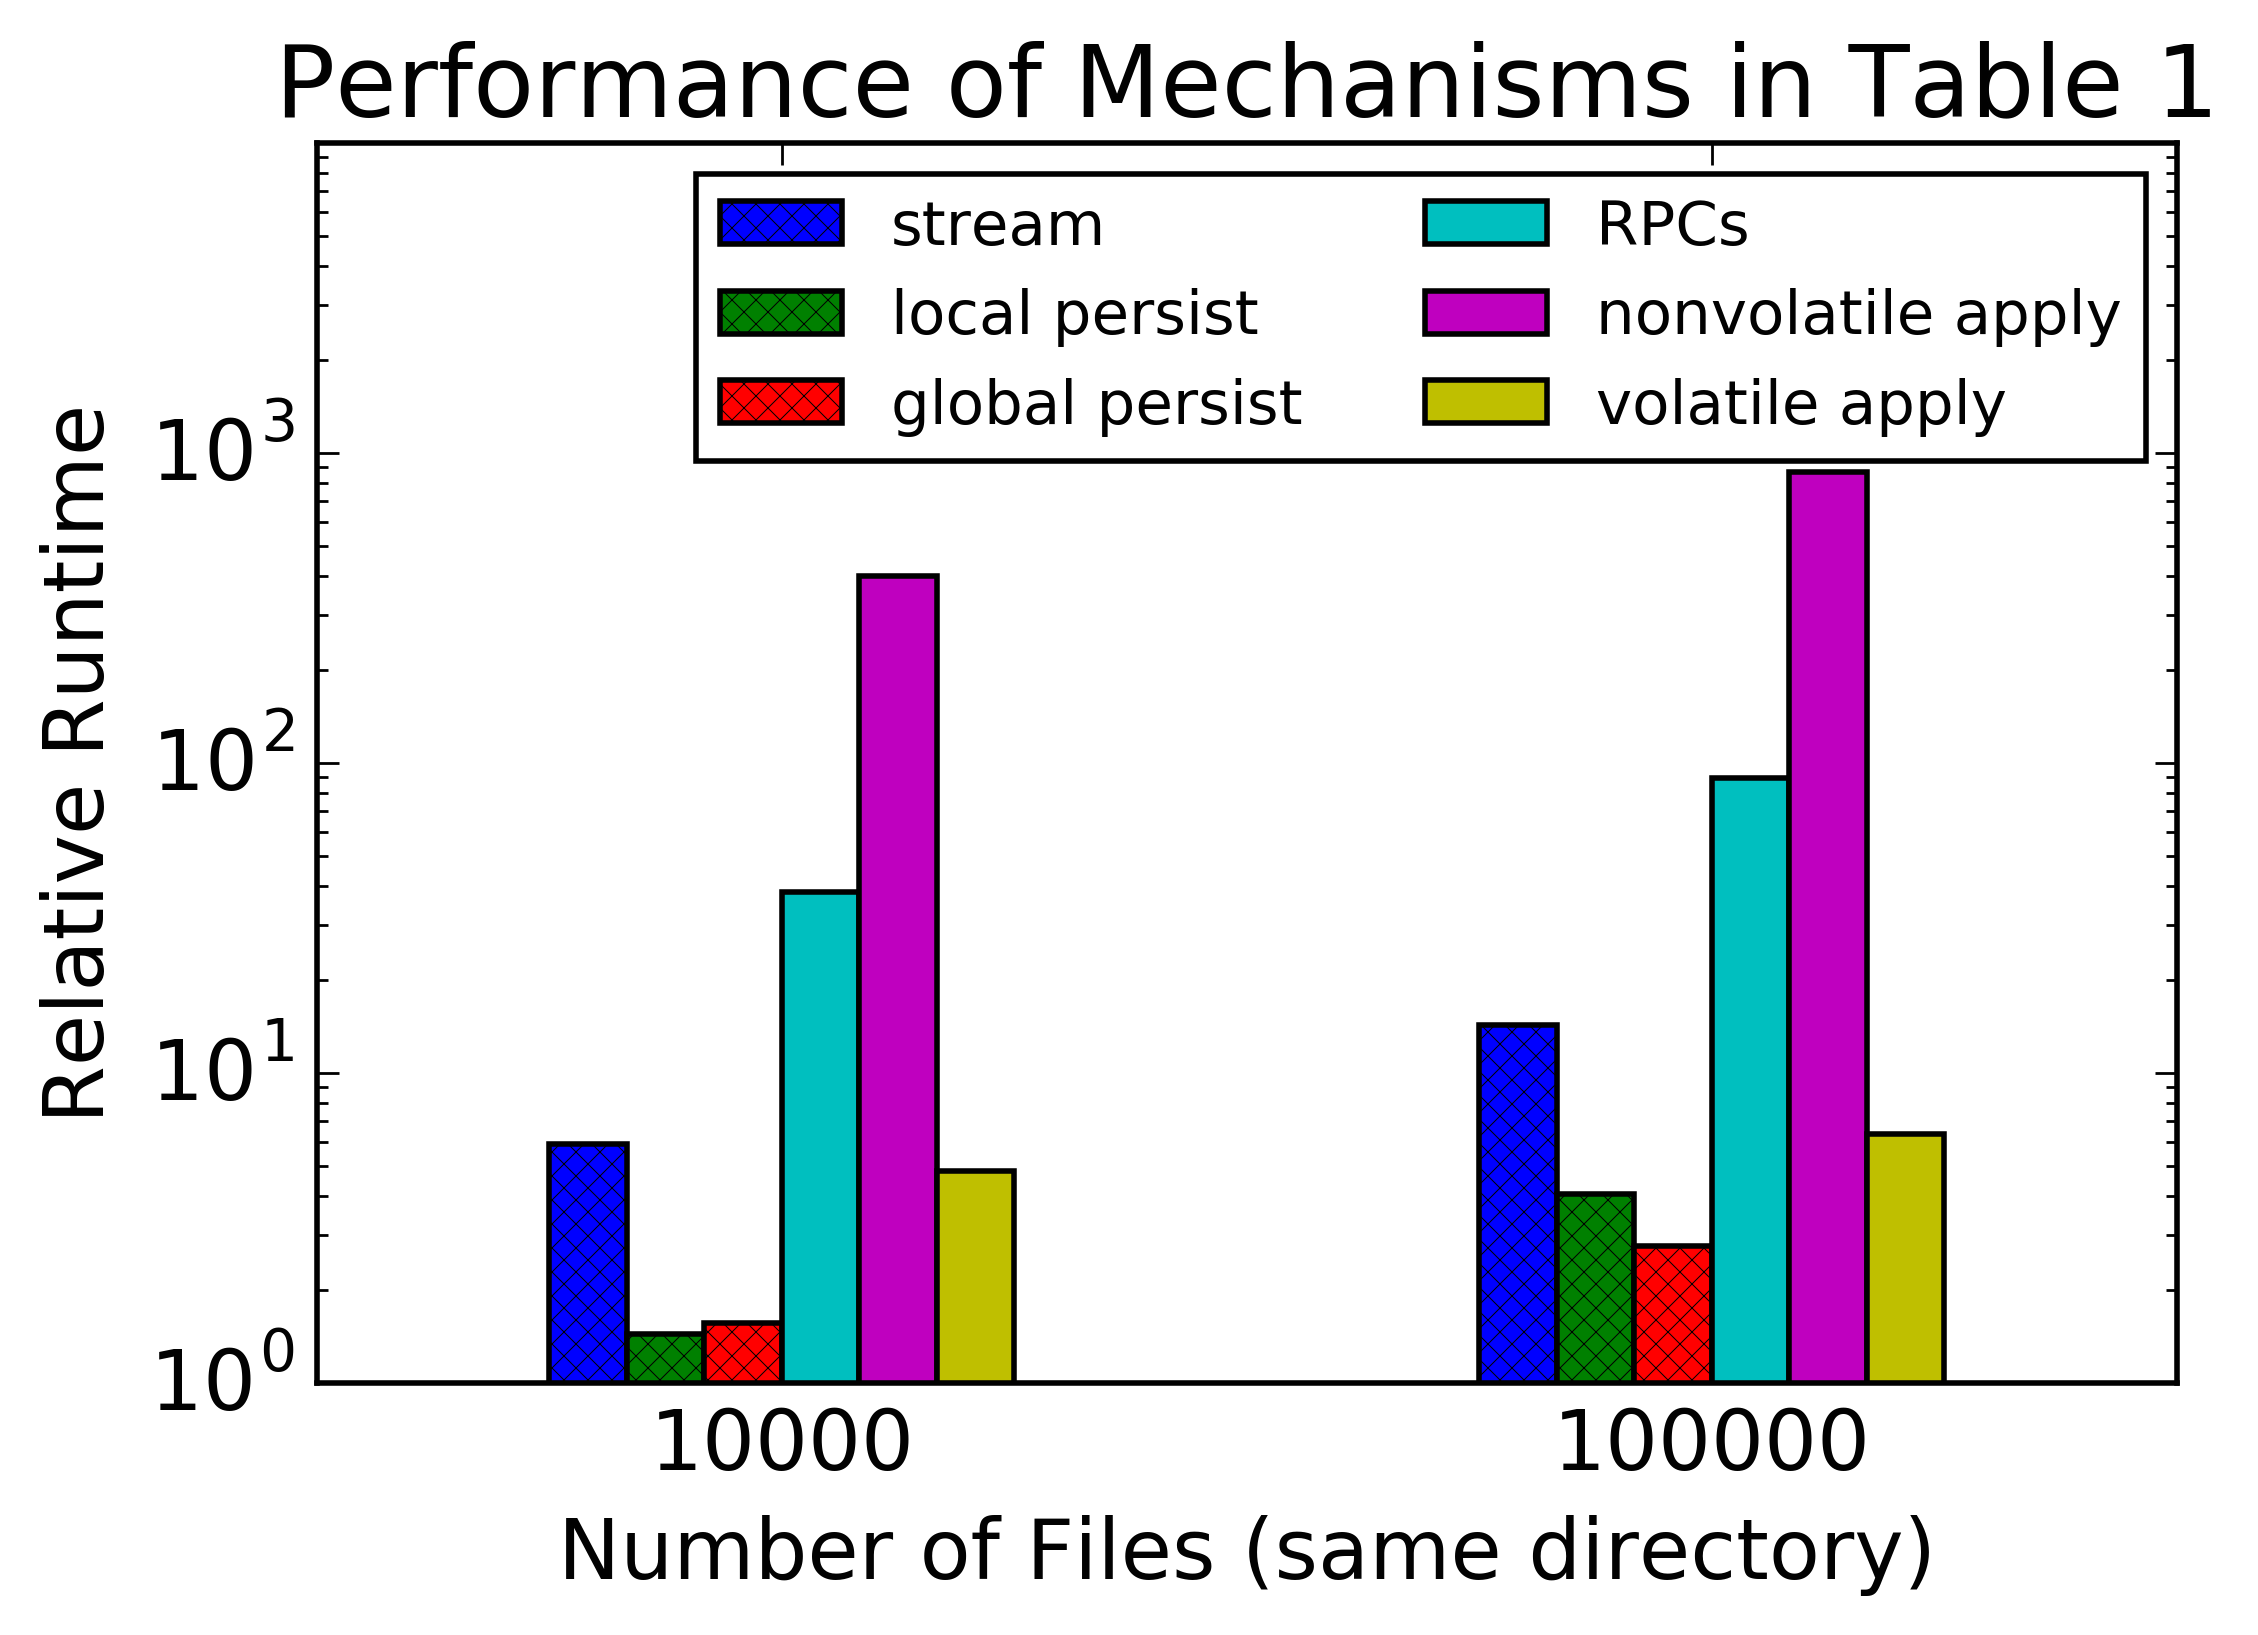
\includegraphics[width=1.0\linewidth]{graphs/slowdown-mechanisms.png}
\caption{
[\href{https://...}{source}]
The performance of the Cudele mechanisms normalized to the runtime of the
``Append Client Journal" mechanism (the runtime of writing \(n\) file creates
to the client's in-memory journal).  \label{fig:slowdown-mechanisms}}
\end{figure}

\begin{figure}[tb]
\centering
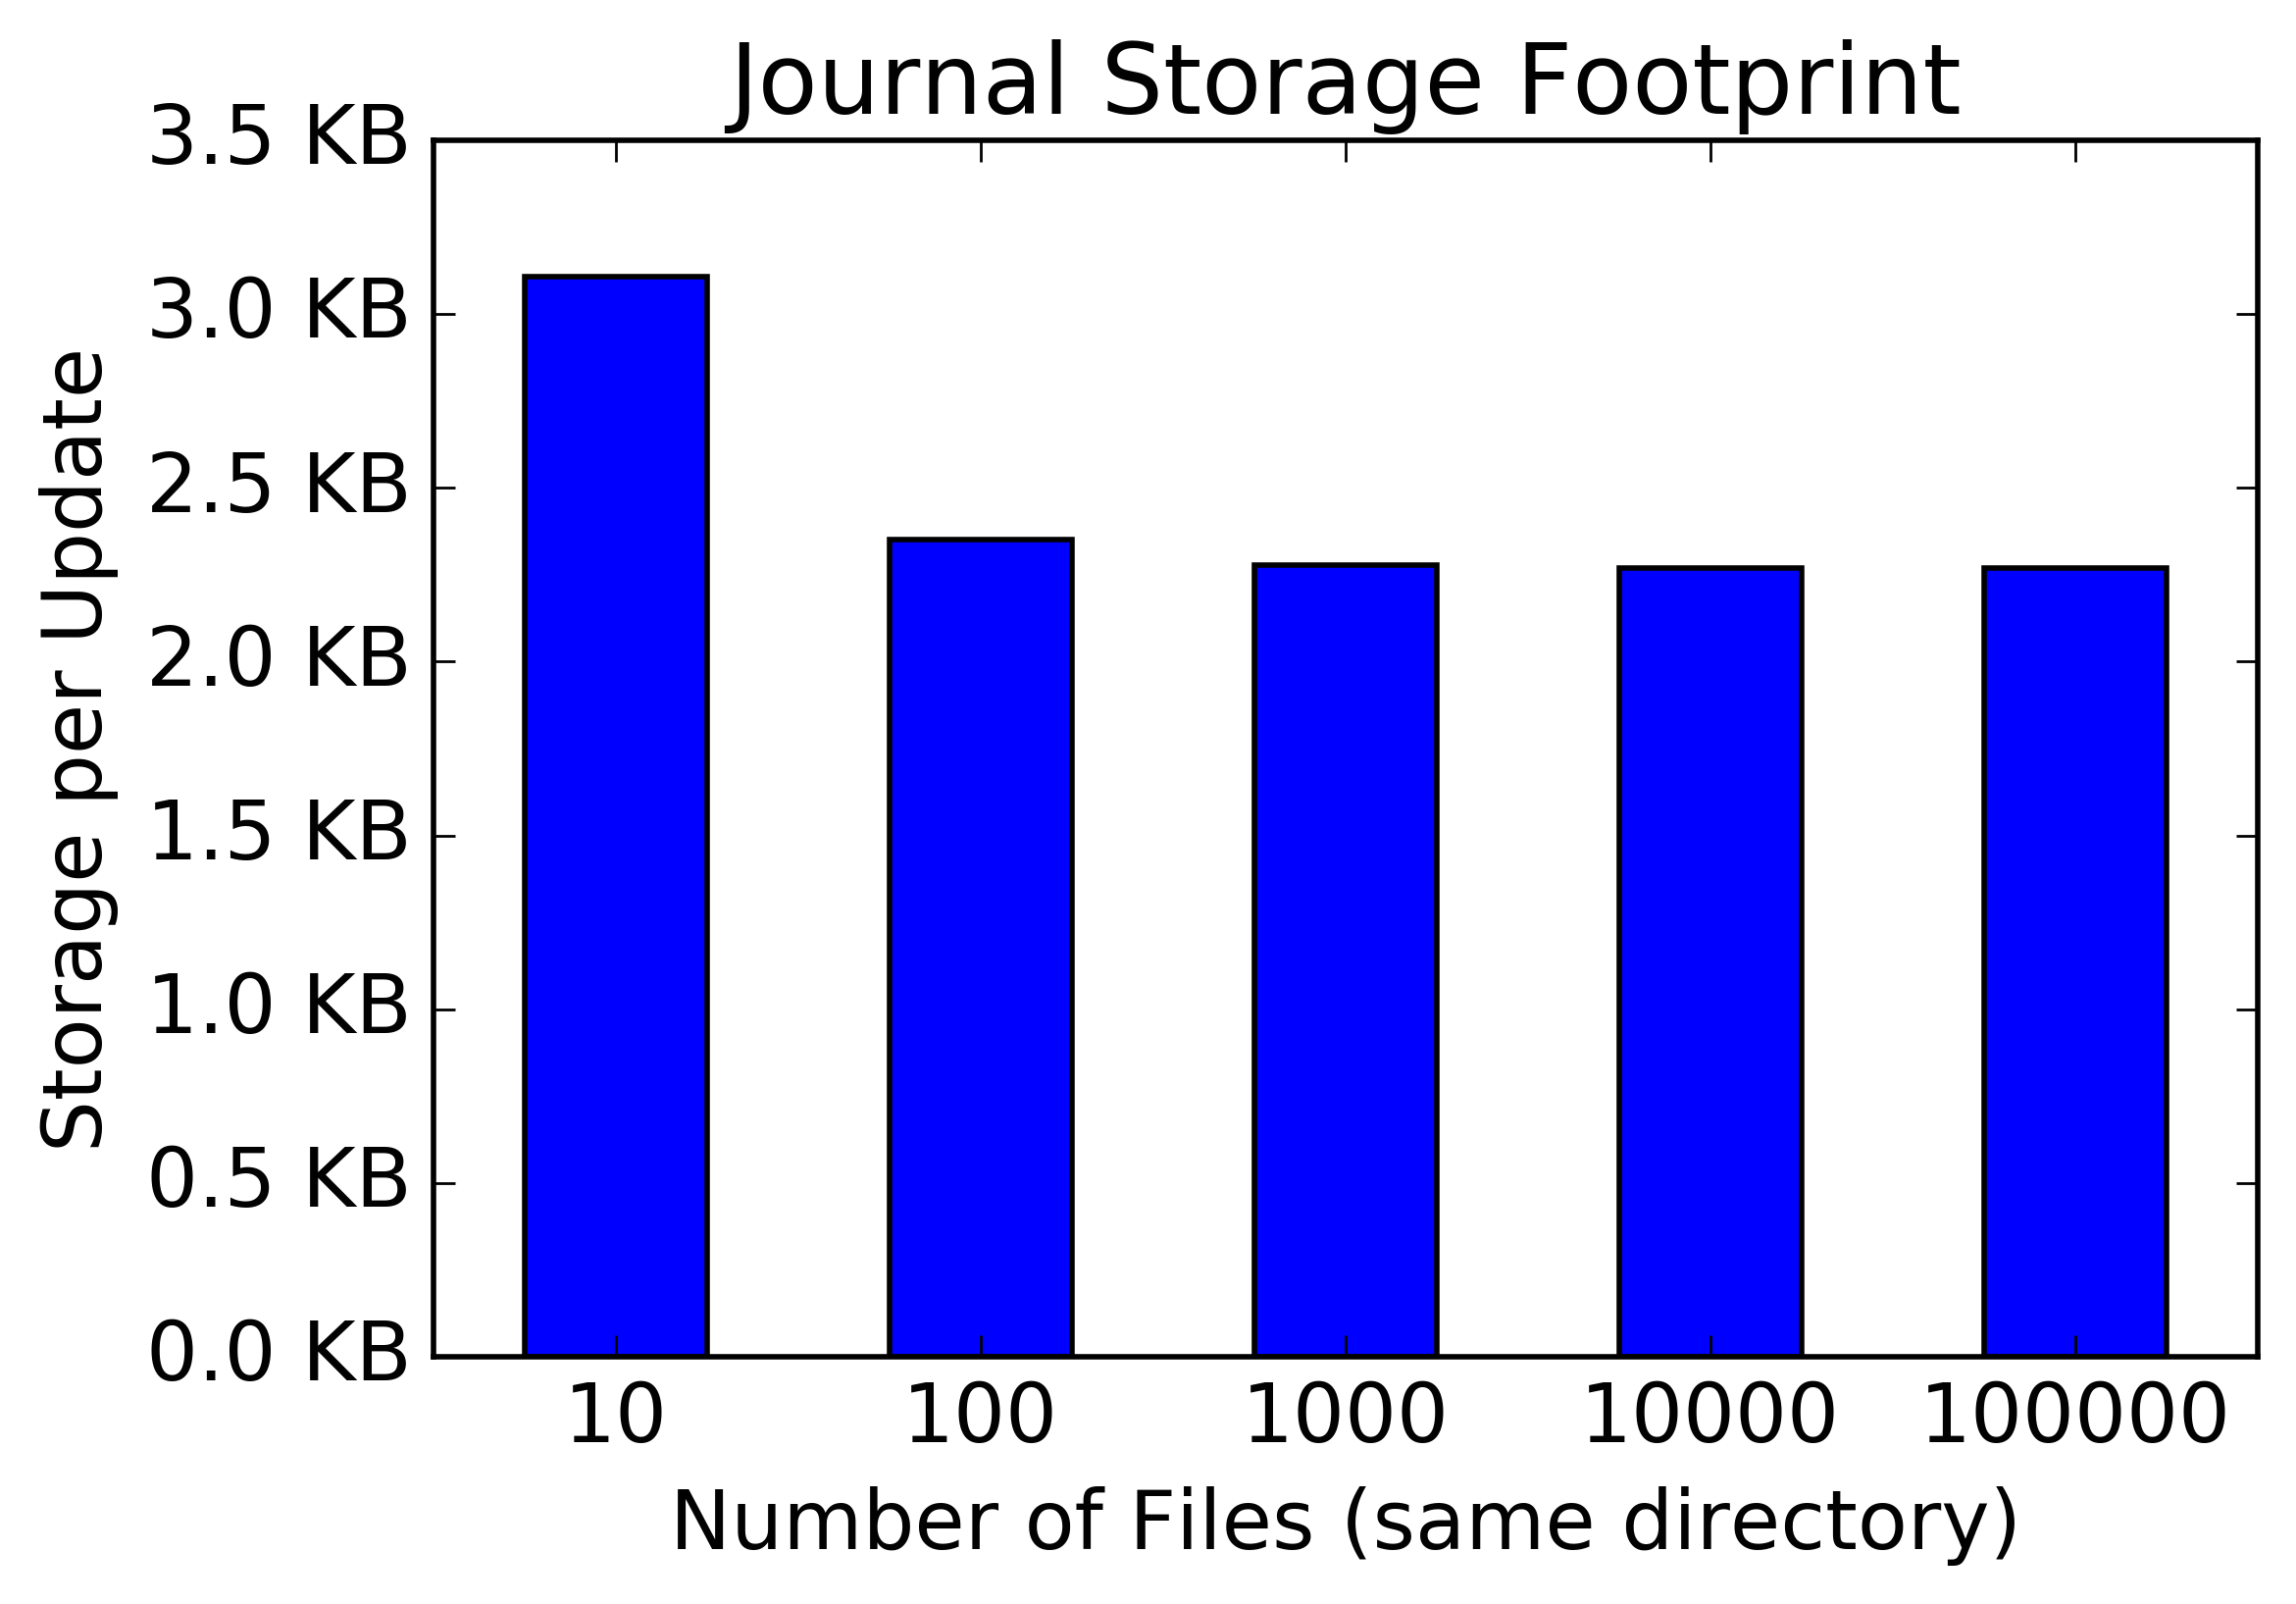
\includegraphics[width=1.0\linewidth]{graphs/behavior-journal-size.png}
\caption{
[\href{https://...}{source}]
The size of the client's journal scales with the number of
updates.\label{fig:behavior-journal-size}}
\end{figure}

Figure~\ref{fig:slowdown-mechanisms} shows the runtime of the Cudele
mechanisms for a single client creating files in the same directory, normalized
to the time it takes to write \(n\) file create updates to the client's
in-memory journal ({\it i.e.} the ``Append Client Journal" mechanism). Bars
above \(10^0\) are slower than the ``Append Client Journal" mechanism.
``Stream" is an approximation of the overhead and is calculated by subtracting
the runtime of the job with the journal turned off from the runtime with the
journal turned on.  The largest workload we tested is 100K file creates in the
same directory.  This is the maximum recommended size of a directory in CephFS;
preliminary experiments with larger directory sizes show memory problems.

{\it Poorly Scaling Data Structures:} Despite doing the same amount of
work, mechanisms that rely on poorly scaling data structures have large
slowdowns for the larger number of creates. For example, ``RPCs" which relies
on the internal CephFS directory structures, goes from a \(40\times\) slowdown
for 10K files to a \(90\times\) slowdown for 100K files. It is a well-known
problem that directory data structures do not scale when creating files in the
same directory~\cite{ren:sc2014-indexfs} and any mechanism that uses these data
structures will experience similar slowdowns. Other mechanisms that write
events to a journal ({\it e.g.} the persists, ``Volatile Apply") experience a
much less drastic slowdown because the journal data structure does not need to
be scanned for every operation. Events are written to the end of the journal without
even checking the validity ({\it e.g.}, if the file already exists for a create),
which is another form of relaxed consistency because the file system assumes the
application has resolved conflicting updates in a different way.

% RPCs vs. apply: calls to metadata server vs. RADOS
{\it Overhead of RPCs:} ``RPCs" is \(66\times\) slower than ``Volatile
Apply" because sending individual metadata updates over the network is costly.
While ``RPCs" sends a request for every file create, ``Nonvolatile Apply"
writes all the updates to the in-memory journal and applies them to the
in-memory data structures in the metadata server. While communicating the
decoupled namespace directly to the metadata server is faster, communicating
through the object store (``Nonvolatile Apply") is \(10\times\) slower.

% TODO: why is apply so slow.  
% apply: no CephFS changes, pulls/pushes same RADOS obj.
% v_apply vs. apply/persist: communicating through RADOS
{\it Overhead of ``Nonvolatile Apply":} The cost of ``Nonvolatile
apply" is much larger than all the other mechanisms.  That mechanism was not
implemented as part of Cudele -- it was a debugging and recovery tool packaged
with CephFS. It works by iterating over the updates in the journal and pulling
all objects that {\it may} be affected by the update.  This means that two
objects are repeatedly pulled, updated, and pushed: the object that houses the
experiment directory and the object that contains the root directory ({\it
i.e.} \texttt{/}).  The cost of communicating through the object store is shown
by comparing the runtime of ``Volatile apply" + ``Global persist" to
``Nonvolatile Apply". These two operations end up with the same final metadata
state but using ``Nonvolatile Apply" is clearly inferior.

% persist vs. save: one disk vs. many
{\it Parallelism of the Object Store:} Comparing ``Local" and ``Global
persist" demonstrates the bandwidth advantages of storing the journal in a
distributed object store. For 100K file creates, the ``Global Persist"
performance is \(1.5\times\) faster because the object store is leveraging the
collective bandwidth of the disks in the cluster. This benefit comes from the
object store itself but should be acknowledged when making decisions for the
application; the size of the object store can help mitigate the overheads of
globally persisting metadata updates.

{\it Journal Size:} Figure~\ref{fig:behavior-journal-size} shows the
amount of storage per journal update (\(y\) axis) for the range of file creates
we tested (\(x\) axis). The increase in file size is linear with the number of
metadata creates and suggests that updates for a million files would be
\(2.5\text{KB}*1\text{ million files} = 2.38\text{GB}\). Transfer times for
payloads of this size on an HPC network are reasonable.\\

\noindent\textbf{Takeaway}: the Cudele mechanisms have overheads and costs
that can differ {\it by orders of magnitude}. Cudele gives users the ability
to compose these mechanisms based on their application's correctness
requirements and performance goals.\\

\begin{figure}[tb]
\centering
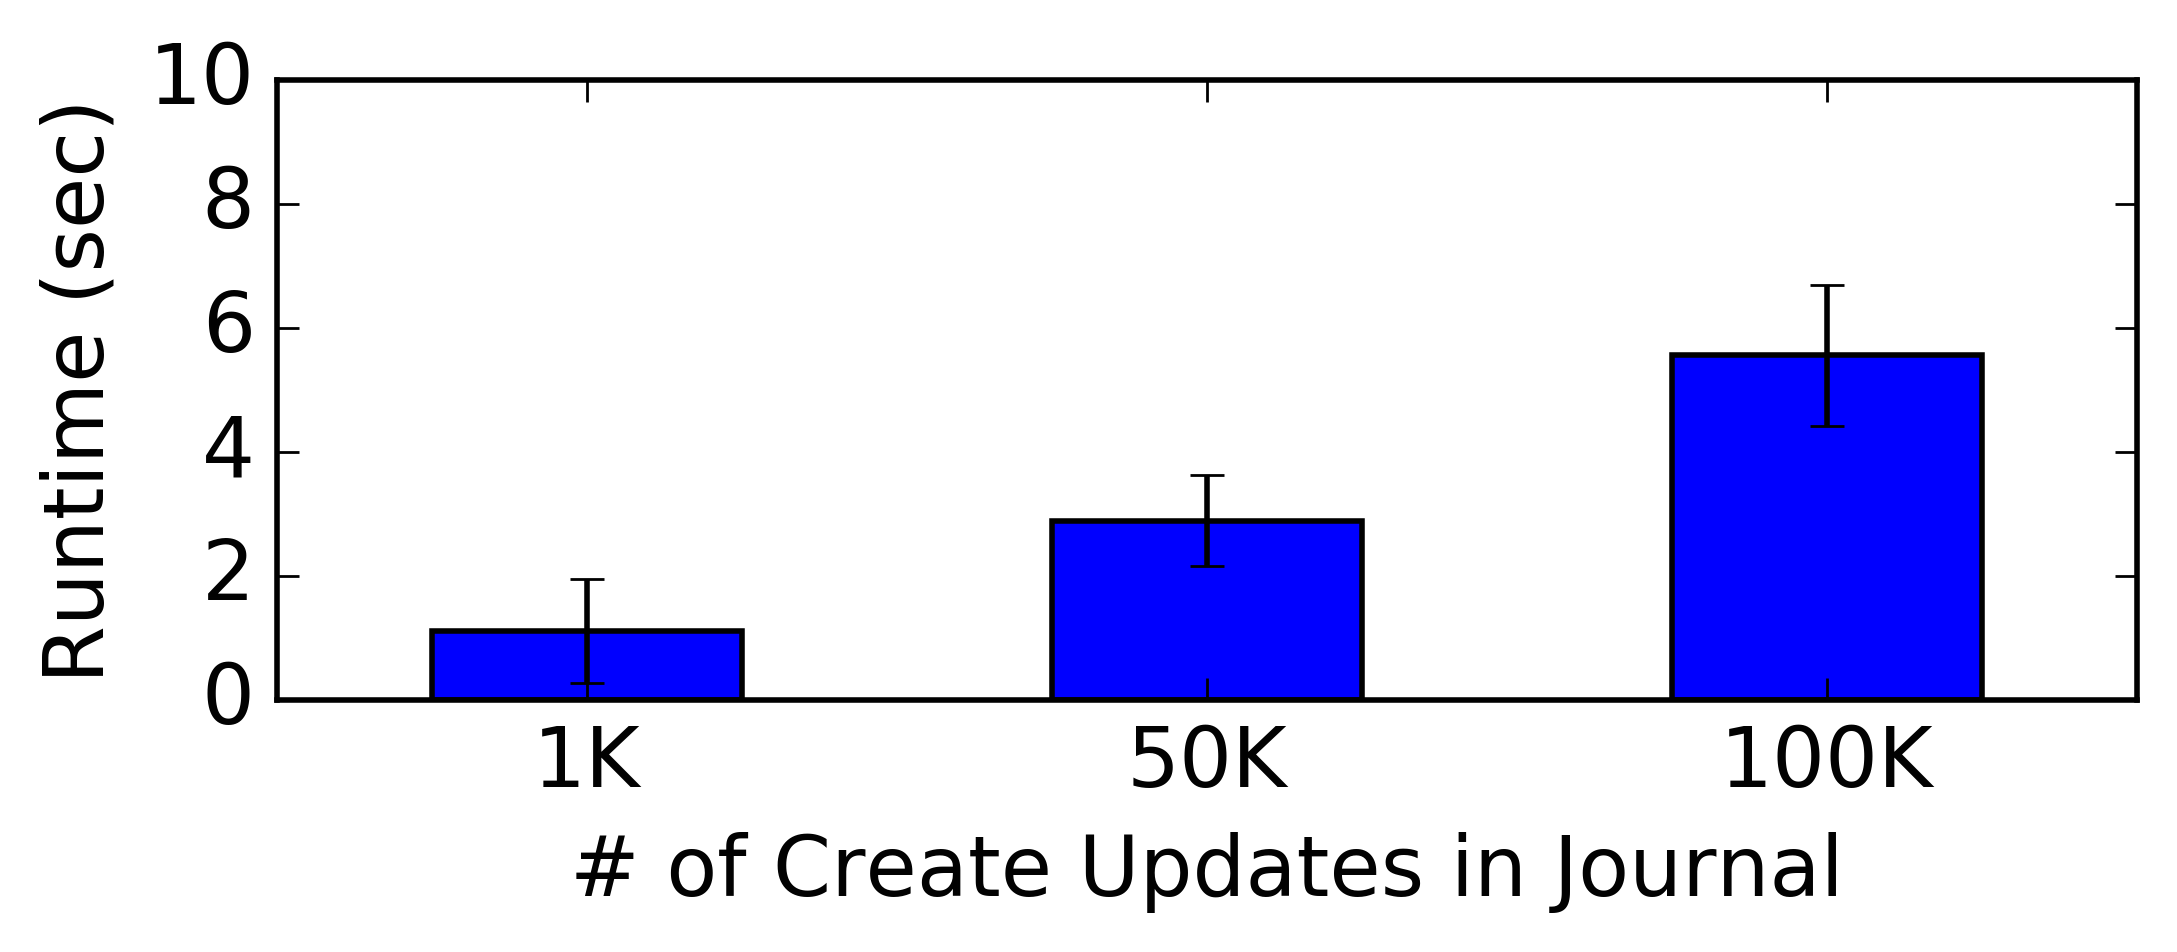
\includegraphics[width=1.0\linewidth]{graphs/merge-a.png}
\caption{ [\href{https://...}{source}] Merging journals serially.}
\label{fig:merge}
\end{figure}

%\begin{figure}[t]
%  \centering
%  \begin{subfigure}[b]{\linewidth}
%      \centering
%      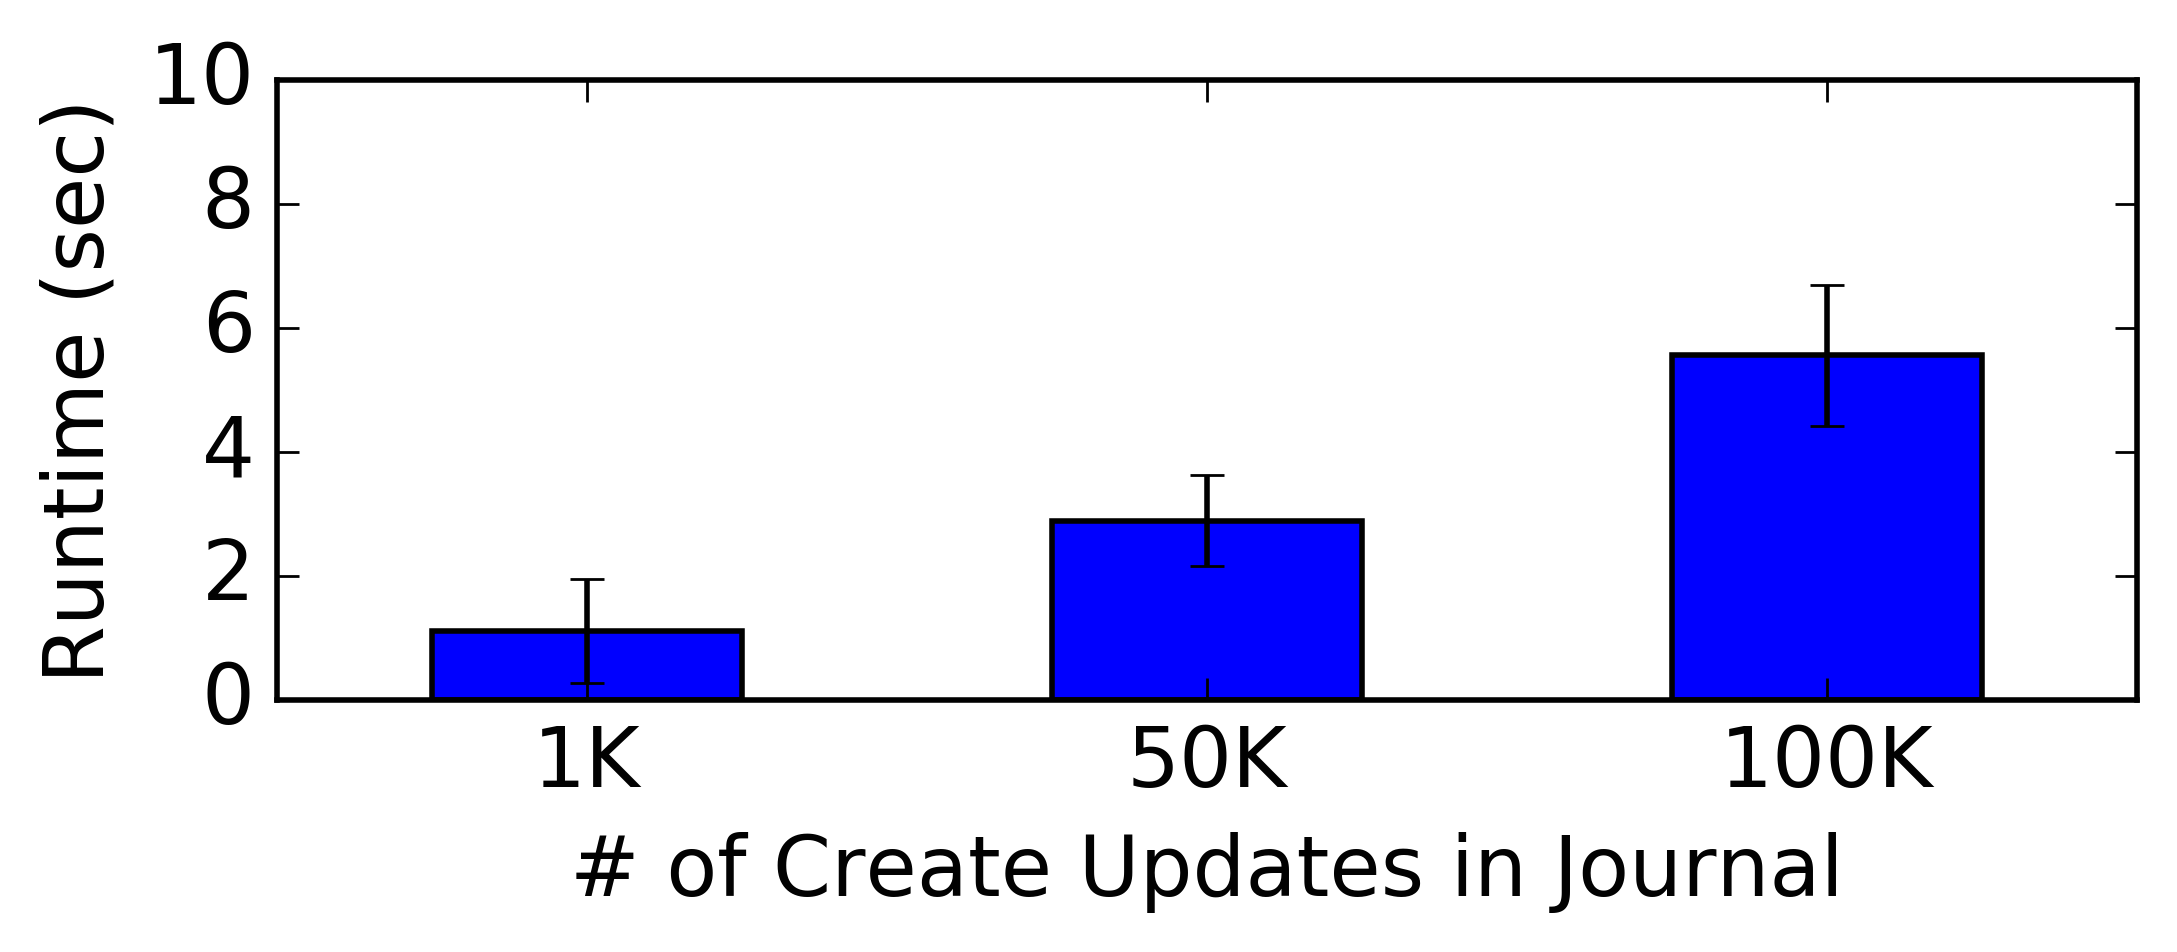
\includegraphics[width=1.0\linewidth]{graphs/merge-a.png}
%      \caption{Merging journals serially.} \label{fig:merge-a}
%  \end{subfigure}\\
%  ~
%  \begin{subfigure}[b]{\linewidth}
%      \centering
%      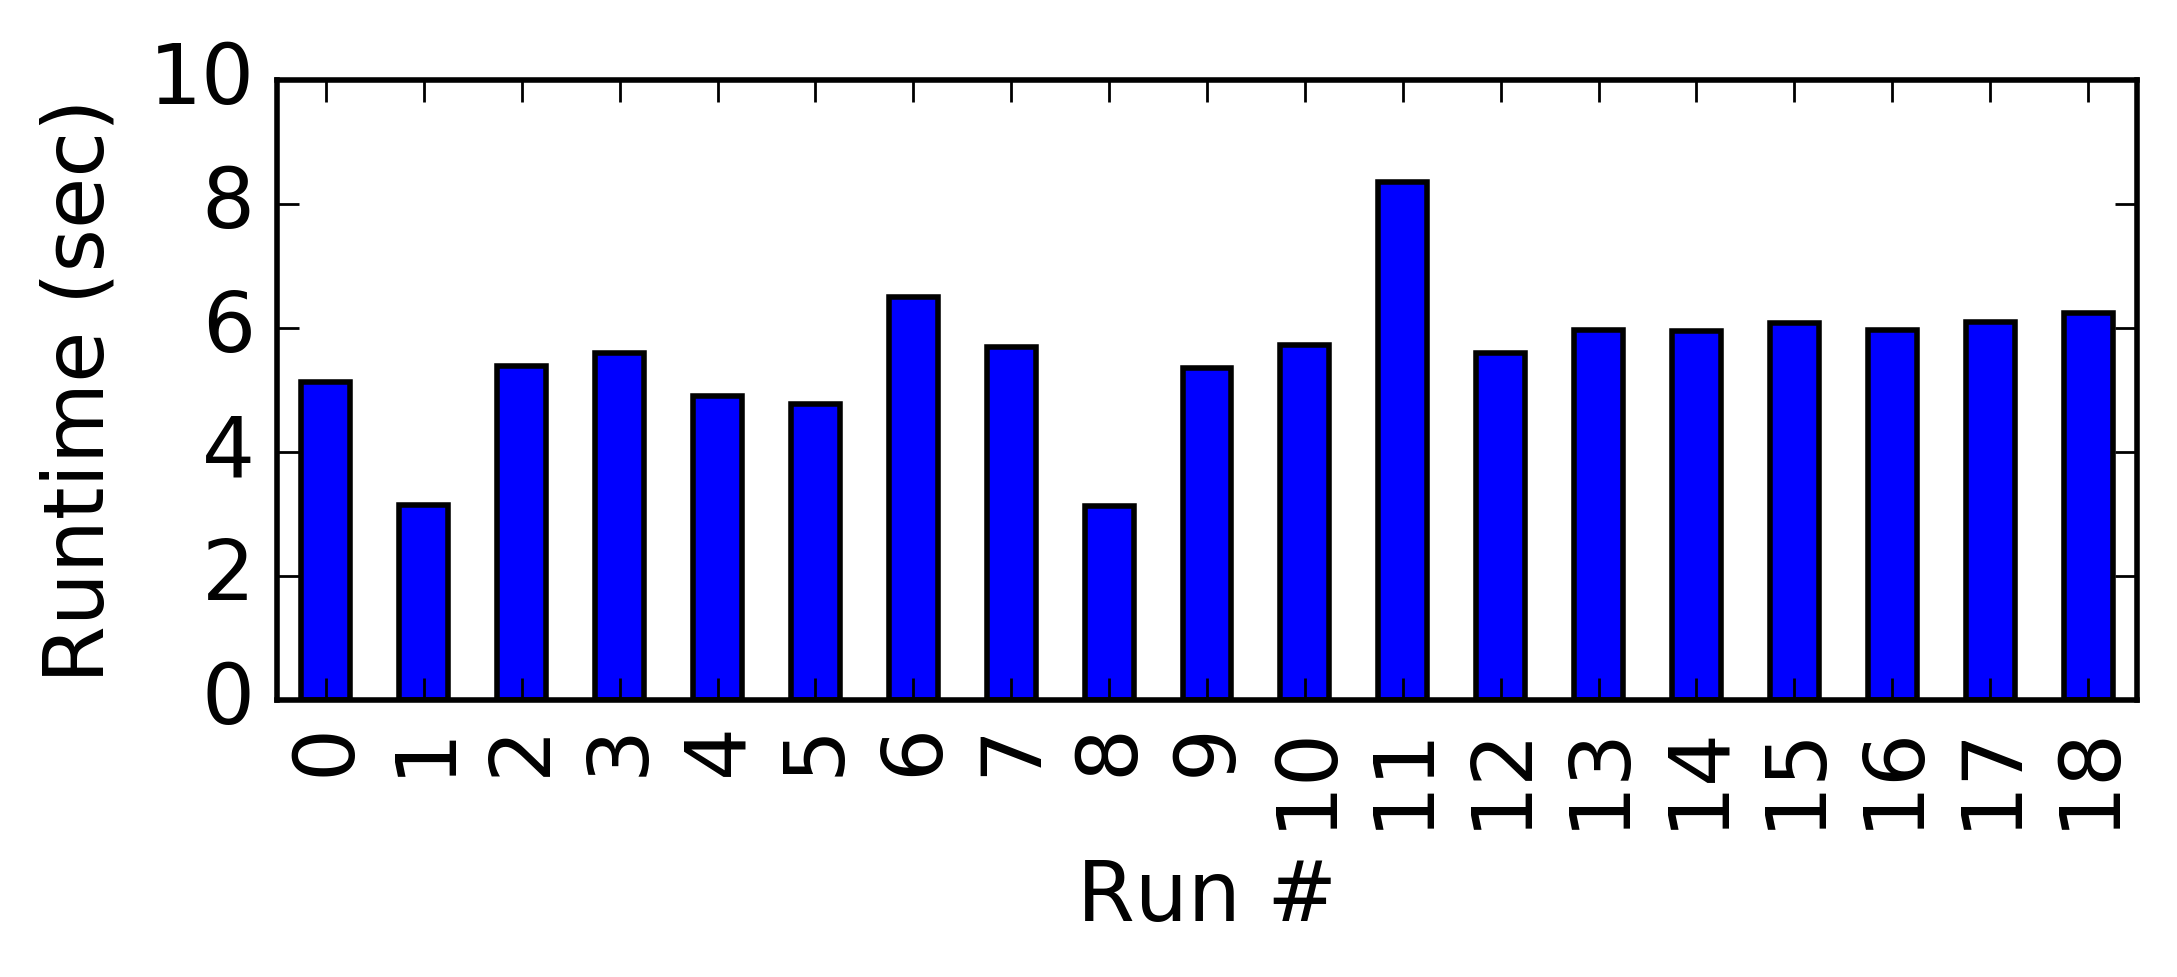
\includegraphics[width=1.0\linewidth]{graphs/merge-b.png}
%      \caption{Merging a journal w/ 100K create updates.}
%      \label{fig:merge-b}
%  \end{subfigure}
%  \caption{Merging updates has linear scalability.\label{fig:merge}}
%\end{figure}

{\it Number of Serialized Merges:} Cudele serializes merge requests at the
metadata server before applying the updates to the in-memory metadata store.
Merging concurrently is an optimization for future work, but merges for the
largest journal size we tested were quite fast.  Furthermore, since we place no
restrictions on the validity of metadata inserted into the journal, we can
avoid touching poorly scaling data structures. In other words, we can scale
linearly if we weaken our consistency by never checking for the existence of
files before creating files.

Figure~\ref{fig:merge} demonstrates this scalability by showing the runtime
(\(y\) axis) of merging journals of different sizes (\(x\) axis). The variance
of the runtime is over 20 serial merges, each hitting a different directory in
the namespace.  The runtime scales linearly and with low variance because the
``Create" mechanism that was used to create the journal only appends
\texttt{open()} requests to the journal. When the updates are merged by the
metadata server into the in-memory metadata store they never scan growing data
structures. Had we implemented the ``Create" mechanism to include
\texttt{lookup()} commands before \texttt{open()} requests, we would have seen
the poor scaling that we see with the ``RPCs" mechanism.\\
%Figure~\ref{fig:merge-b} confirms that we do not touch a poorly scaling data
%structure because the runtimes do not increase as we add more metadata. \\

\noindent\textbf{Takeaway}: the weakest form of consistency for creating files
({\it i.e.} not checking data structures for the validity of an update or
existence of a file) shows linear scalability and stable performance.



\subsection{Use Case 1: Creates in the Same Directory}
\label{use-case-1}

% CITEME xiao:socc2015-shardfs CITEME HADOOP
Clients creating files in private directories is heavily studied in
HPC~\cite{weil:sc2004-dyn-metadata, ren:sc2014-indexfs, patil:fast2011-giga,
zheng:pdsw2014-batchfs, sevilla:sc15-mantle}, mostly due to
checkpoint-restart~\cite{bent_plfs_2009}.  But the workload also appears in
cloud workloads, where systems like Hadoop use the file abstraction to exchange
work units to workers or to indicate when jobs
complete~\cite{shvachko:login2012-hdfs-scalability}. A more familiar example is
uncompressing an archive ({\it e.g.}, \texttt{tar xzf}), where the file system
services a flash crowd of creates across all directories as shown in
Figure~\ref{fig:overhead-creates}.  We use this as a microbenchmark because it
allows us to control the size of the log, since each create creates a single
journal event.

\begin{figure}[tb]
\centering
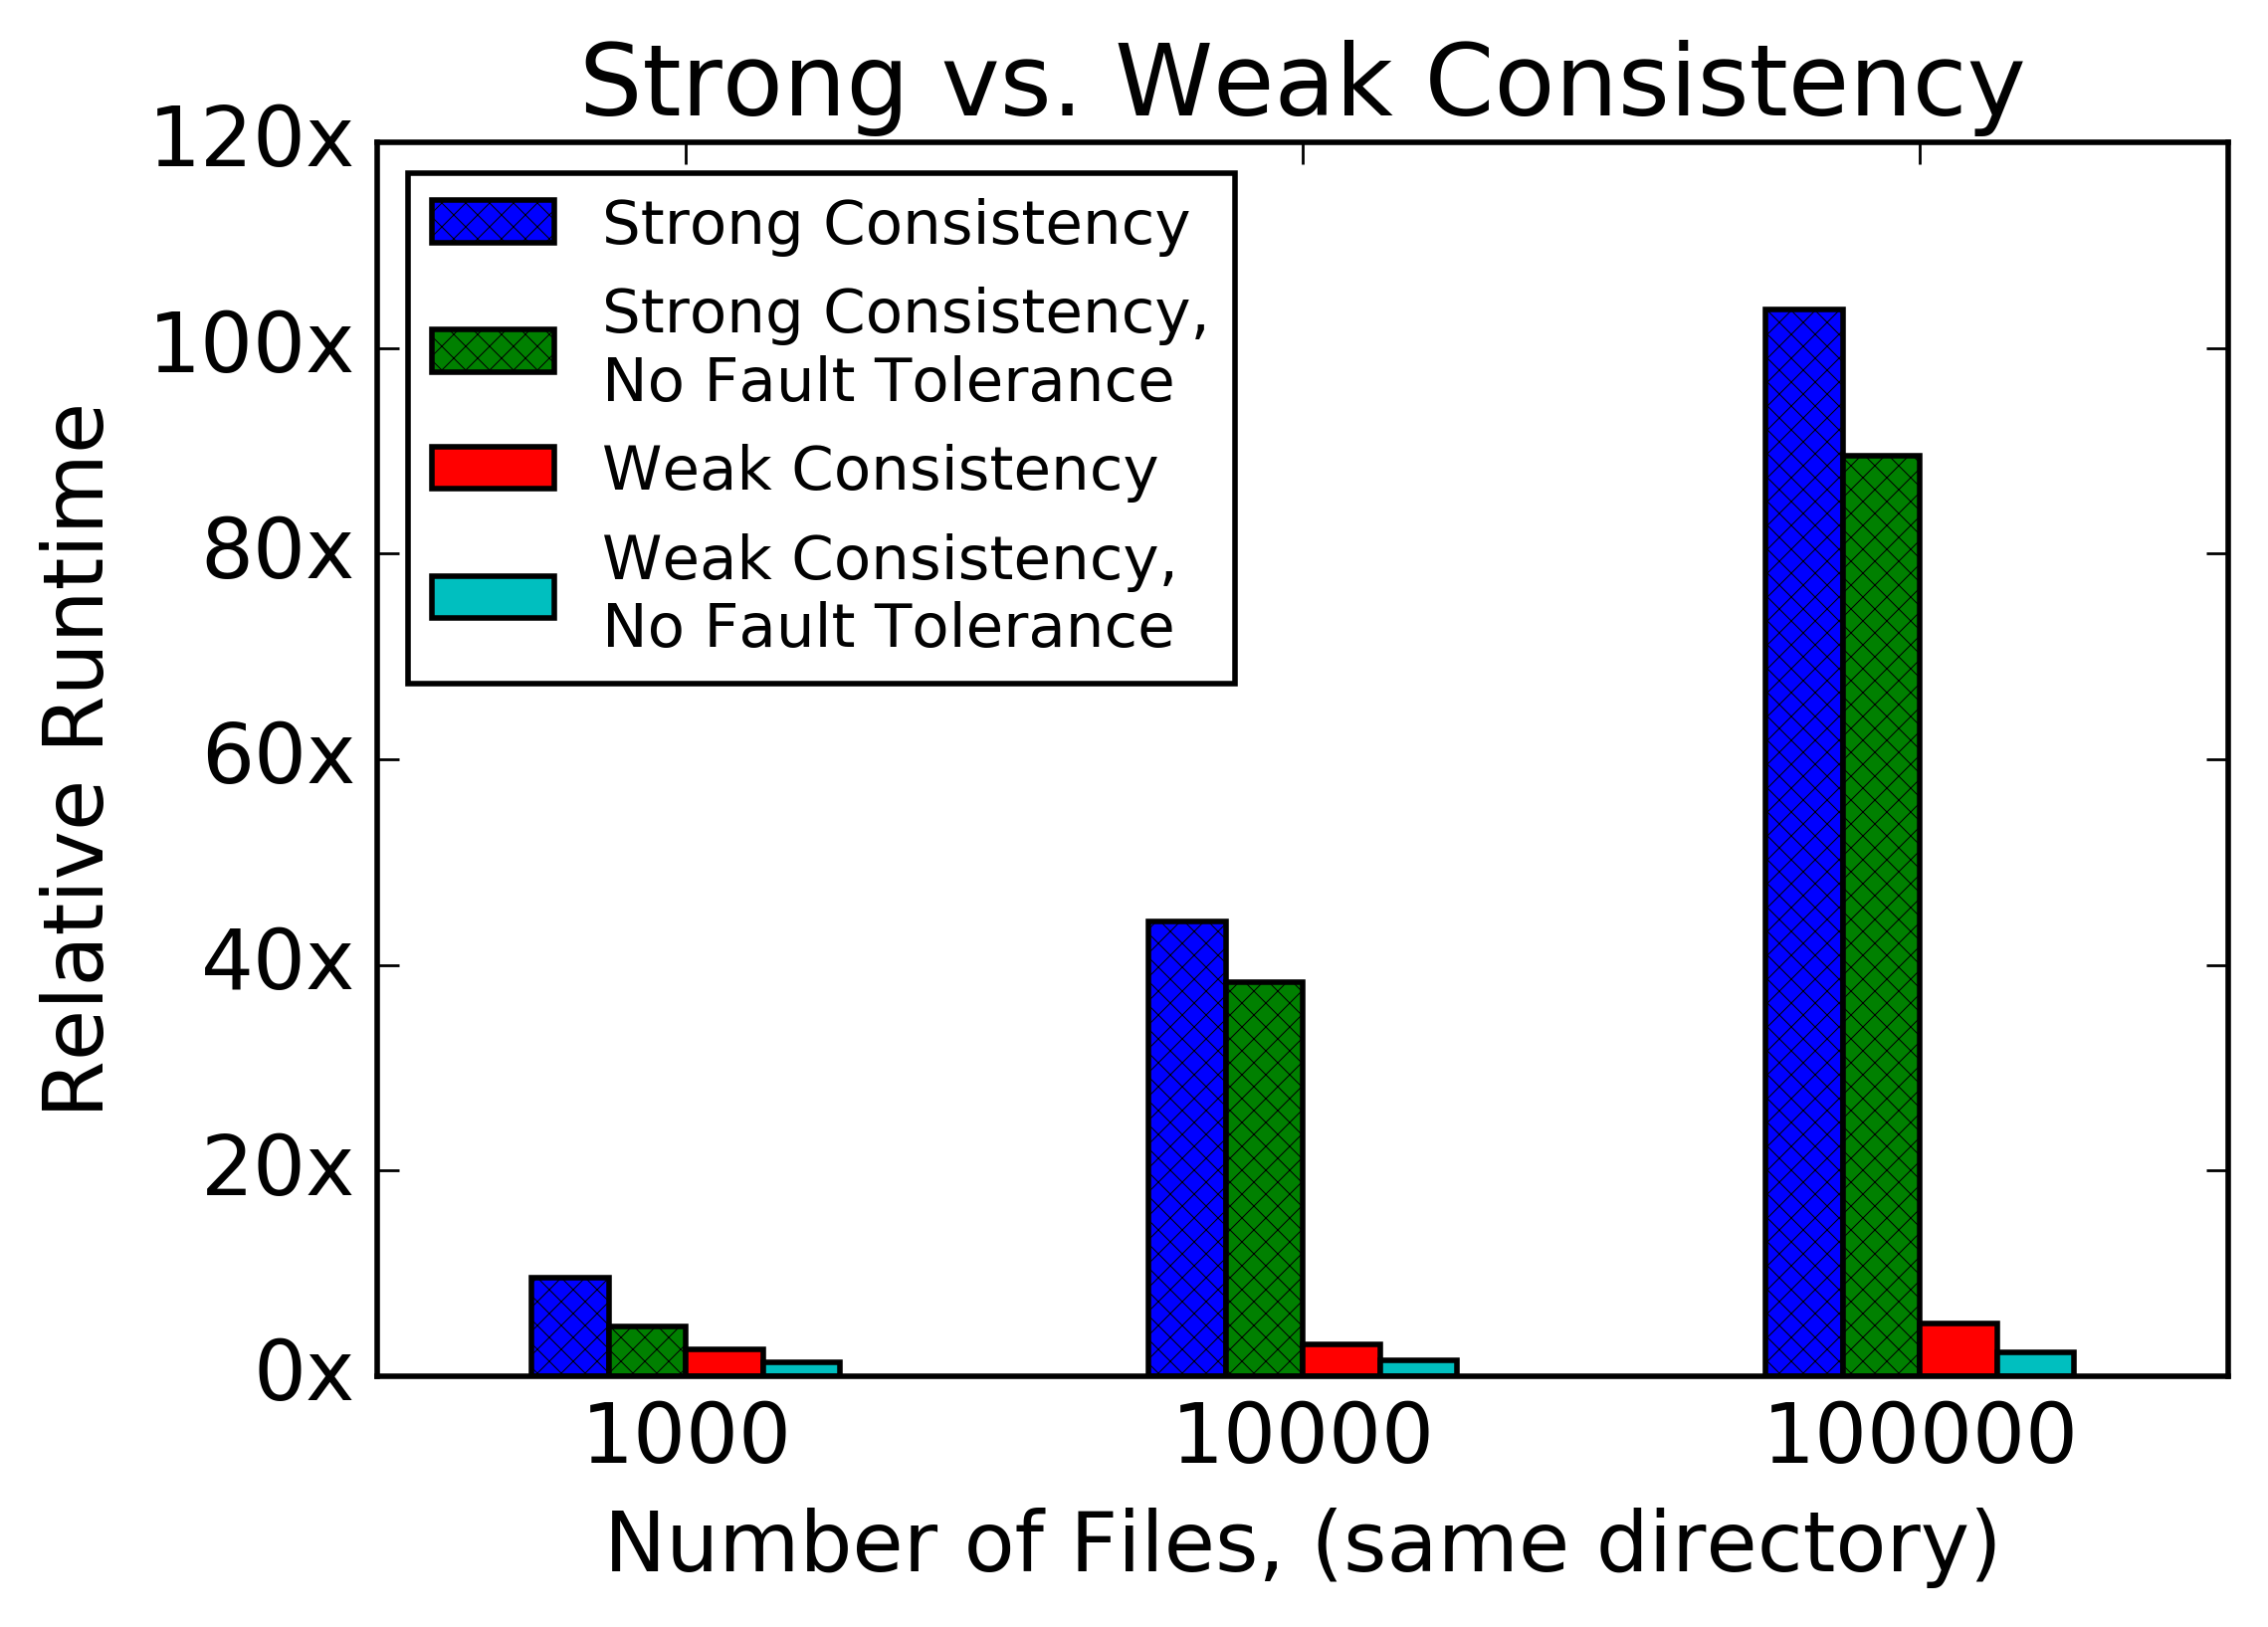
\includegraphics[width=1.0\linewidth]{graphs/slowdown-strong-v-weak.png}
\caption{
[\href{https://...}{source}]
The RPC per metadata update of ``Strong Consistency" has a large
overhead compared to the decoupled namespace strategy of ``Weak
Consistency".\label{fig:slowdown-strong-weak}}
\end{figure}

Figure~\ref{fig:slowdown-strong-weak} shows the runtime of systems employing
weak and strong consistency, normalized to the runtime of the ``Append Client Journal"
mechanism (again, just creating files in the client's in-memory journal).  We
use the following compositions from the mechanisms in
Table~\ref{table:spectrum}:  Strong Consistency = ``RPCs" + ``Stream"; Strong
Consistency, No Fault Tolerance = ``RPCs"; Weak Consistency = ``Append Client Journal" +
``Local Persist"; and Weak Consistency, No Fault Tolerance = ``Append Client Journal" +
``Local Persist" + ``Volatile Apply".

% Final file system metadata states are equivalent No guarantees while
% transitioning mechanisms
We compare these semantics because the final metadata states are equivalent.
Cudele makes no guarantees during execution of the mechanisms or when
transitioning semantics -- the semantics are guaranteed {\it once the mechanism
completes}. So if servers fail during a mechanism, metadata or data may be
lost.

% DeltaFS vs. BatchFS vs. POSIX: decoupled is faster
% (5-7x) vs. (90-104x) slower
% Does not scale?
% Strong Consistency > 10X slower than Weak Consistency 
{\it Speedups of Decoupled Namespaces:} Weak consistency uses the
decoupled namespace strategy and shows up to a \(20\times\) speedup over the
traditional namespaces that use RPCs. Compared to the baseline the slowdown is
\(5-7\times\) for Strong Consistency, which emulates BatchFS and
\(90-104\times\) for Weak Consistency, which emulates DeltaFS.

% POSIX (no stream) vs. POSIX: cost of durability < consistency
{\it Durability \(<<\) Consistency:} The \(1.15\times\) overhead of
Strong Consistency compared to Strong Consistency, No Fault Tolerance for
100K files is negligible. It suggests that the overhead of consistency is much
larger than the overhead of durability. This conclusion should be stronger as
we scale the number of files because the cost of streaming the journal into the
object store is constant. We omit the same analysis for Weak Consistency
because the runtimes are so short that the normalized slowdowns are misleading.

% Weak Consistency benefit not due to metadata format
{\it Metadata Formats:} Because the metadata formats are the same for
all schemes we argue that the performance gain for decoupled namespaces comes
from relaxing the consistency guarantees and not from the metadata formats.\\

\noindent\textbf{Takeaway}: Cudele shows the true benefit of eventual
consistency, where we see over a \(100\times\) slowdown for achieving strong
consistency, in the worst case.

%\section{notes}
%Linking clients into our custom libcephfs
%
%Use namespace's recursive data structure to put policies on subtrees
%- consistency: weak vs. strong, global vs. local
%  - e.g., BatchFS/DeltaFS: weak, local
%  - e.g., POSIX: strong, global
%  - e.g., PLFS: no consistency
%- durability: global vs. local
%  - e.g., CephFS: global
%  - e.g., BatchFS/DeltaFS: local
%
%Experimental Setup
%- Ceph: 9 OSDs, 1 metadata server, 2 kernel client
%- Workload limitations: blah
%
%Workload: creates
%
%Baseline: 200K creates in the same directory
%- throughput: degrades at 950s
%- CPU utilization: more at 950s
%- inode cache: eviction dominate
%- inodes +- to cache: eviction dominate
%- per-disk throughput: RADOS not bottleneck
%
%Experiment 1: Interference
%
%\subsection{Baseline}
%Experiment 0: creates in the same directory
%- setup: why we use caching, we use the kernel client, how we circumvent max fragment size
%
%Experiment 0: creates with a stat
%- Hypothesis: metadata read pauses creates and requires a snapshot in time
%  - what is more of an overhead: pausing creates and getting a consistent view OR sucking up resources as it reads from RADOS?
%- can we delay snapshot?
%
%Experiment 1: creates with a readdir
%- Hypothesis: shows the cost of synchronization because on a write, the first client drops his caps
%- client0: create 100k, client1: stat at 2 mins
%
%Experiment 2: scale the number of files
%- See if the open/close spike occurs 
%- Try to see why open/close spike is allowed to happen
%- Try to disable all caching -- metadata writes don't ever re-use the inode -- we never ask for it again!
%- client0: create 100k, client1: touch at 2 mins
%
%Experiment 3: see how fast the cache satisfies a read
%- client0: create 100k, stat inodes
%- client0: create 100k, client1: stat inodes
%
%lient 0: creates, client 1 create(s)

\subsection{Use Case 2: Creates with Rogue Client}

Clients create files in private directories and a separate client, which we
call a ``rogue" client, creates files in each directory. This introduces false
sharing and the metadata server revokes capabilities on directories touched by
the rogue client. While HPC tries to avoid these situations with
worklflows~\cite{zheng:pdsw2014-batchfs, zheng:pdsw2015-deltafs}, it stills
happens in distributed file systems when users unintentionally access
directories in a shared file system.

\begin{figure}[tb]
\centering
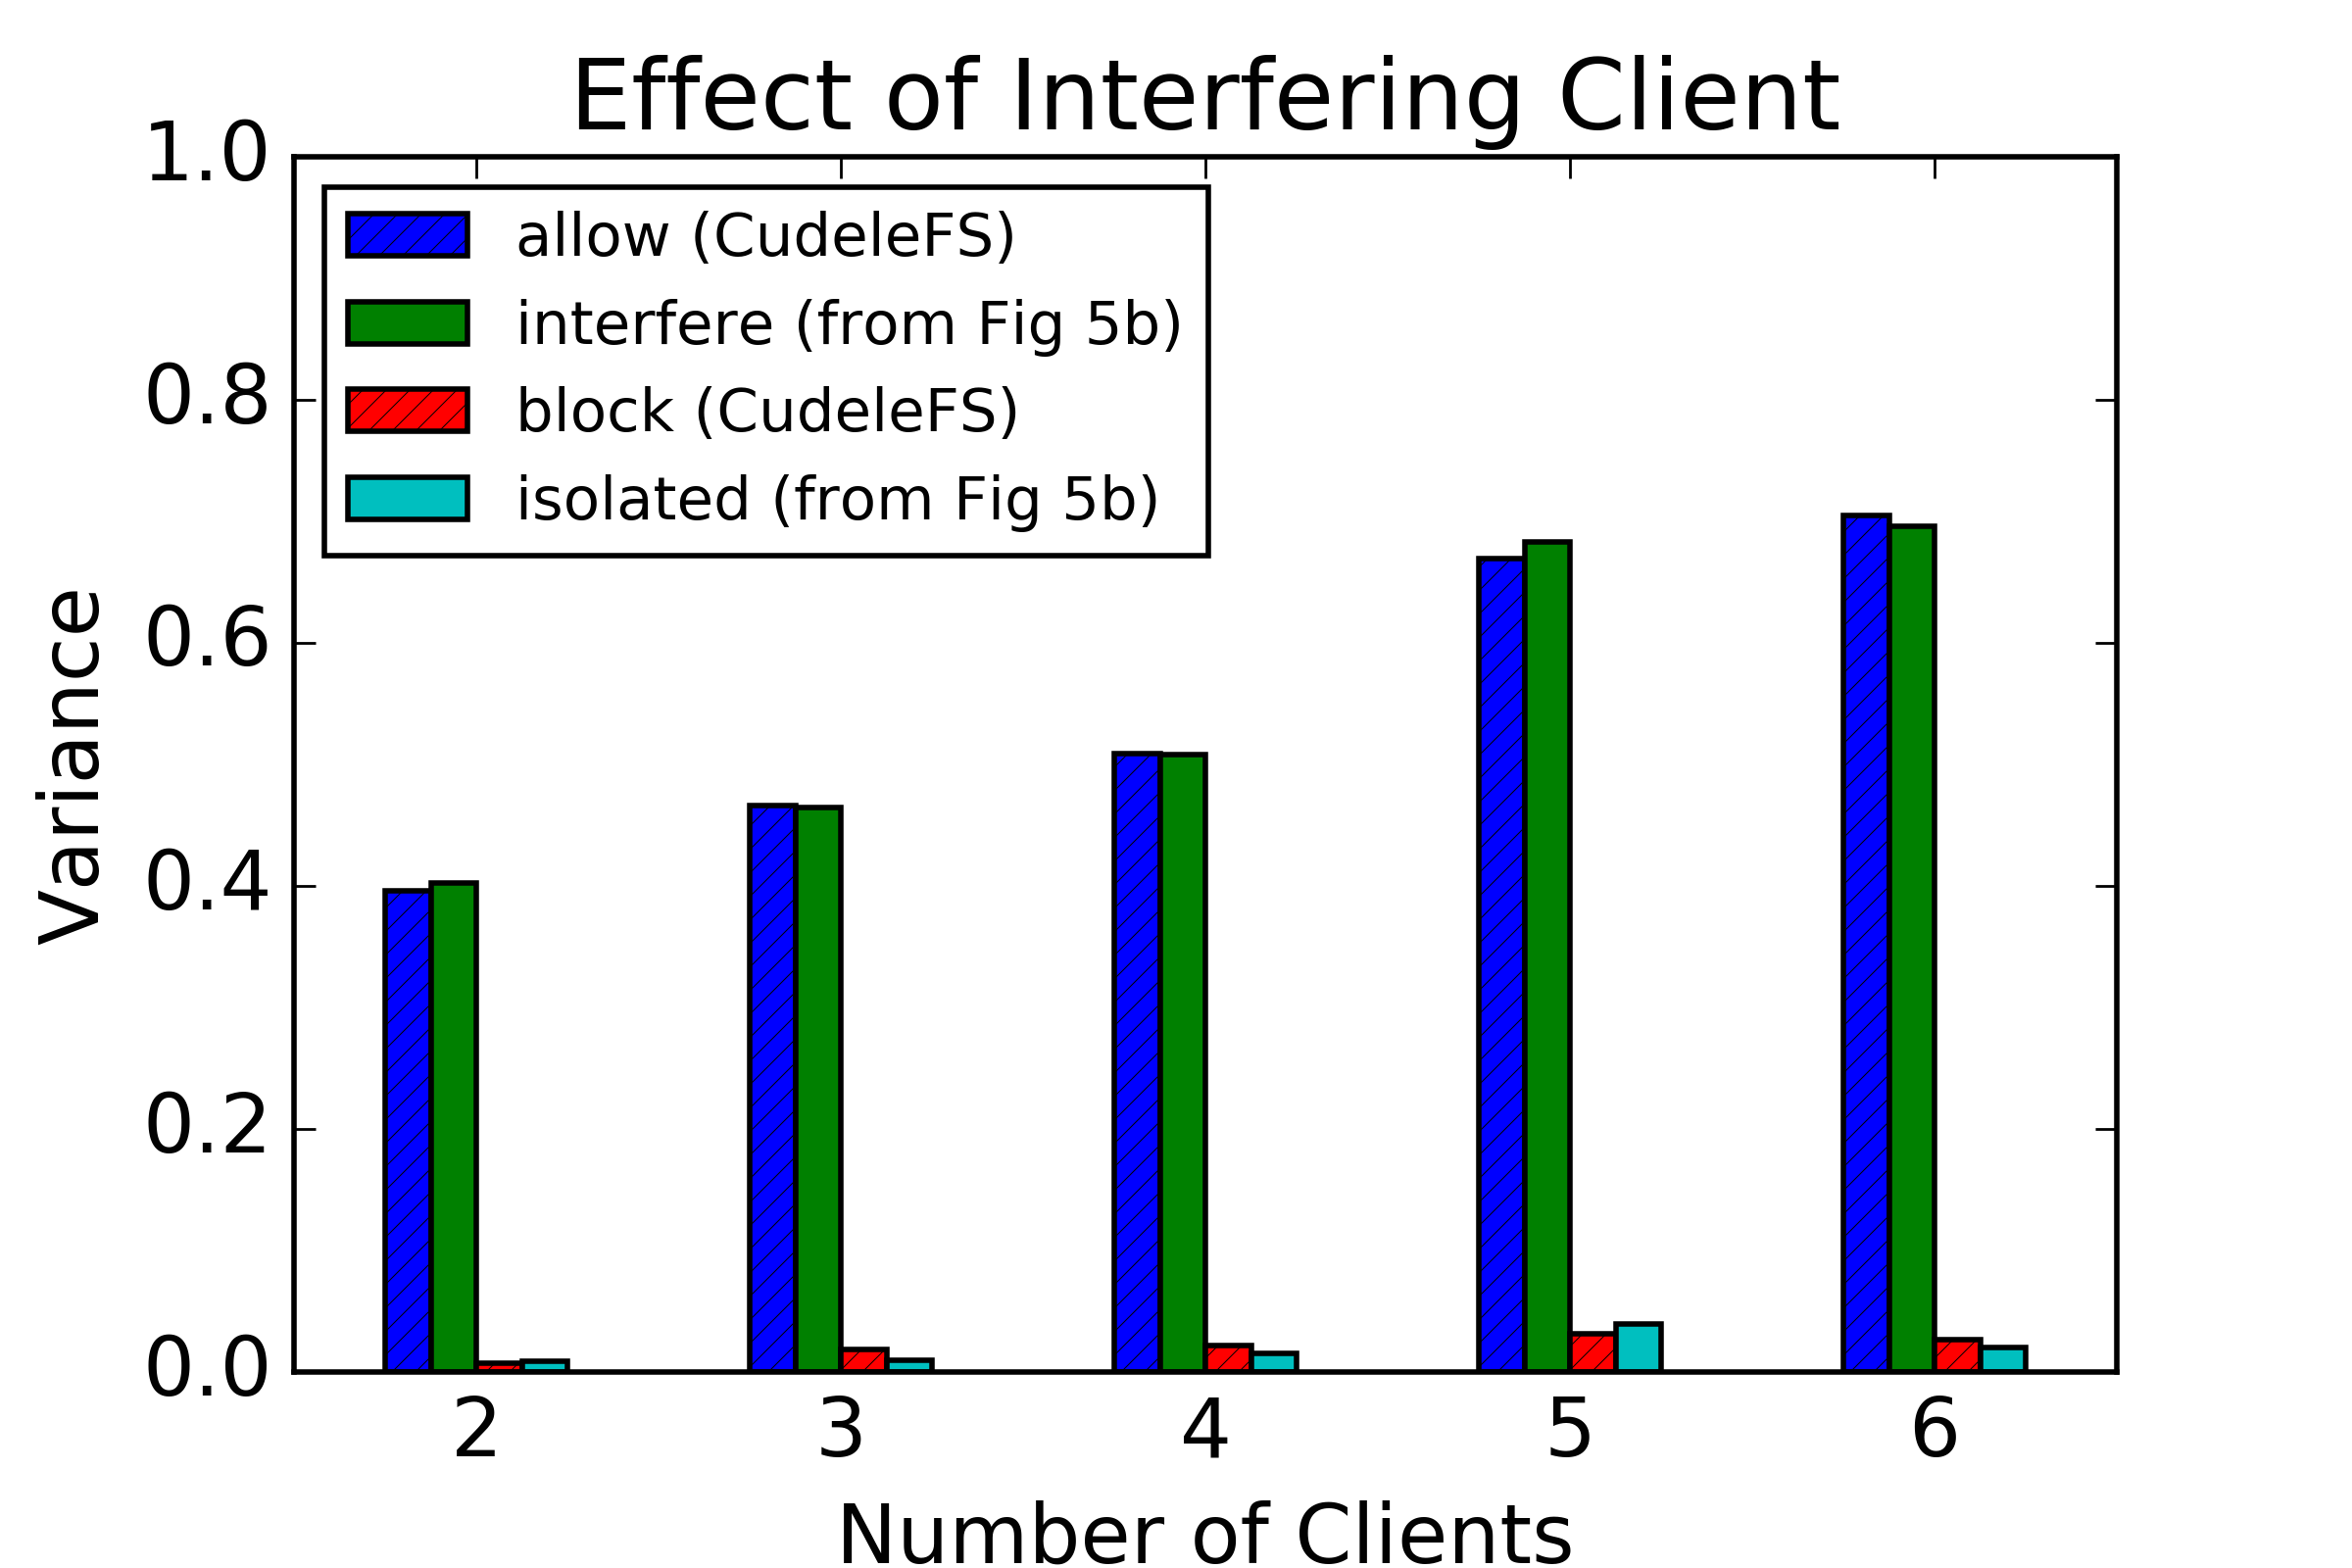
\includegraphics[width=1.0\linewidth]{graphs/slowdown-allow-block.png}
\caption{
[\href{https://...}{source}]
Using the ``allow" and ``block" API, users can isolate directories from
interfering clients. Variance with blocking turned on is the same as
``isolated" from Figure~\ref{fig:overhead-b}.
\label{fig:slowdown-allow-block}}
\end{figure}

% setup: 2cs sep dirs, 2cs DN, 1c malicious write
Next we show how Cudele can be programmed to block interfering clients. We
use the same problematic workload from Figure~\ref{fig:overhead-b}, where
clients write to their own private directories and another client interferes with a stream of creates at
30 seconds.  We also have another client write to a decoupled namespace and
merge its updates at 90 seconds.  We equip each client directory with the
configuration:

\begin{listing}[tb]
\begin{minted}[xleftmargin=21pt,
               tabsize=4]{js}
{     
    "allocated_inodes": "100000"
    "interfere_policy": "block"
    "consistency": "RPCs"
    "durability": "stream"
}
\end{minted}
\end{listing}

Each directory functions with ``RPCs"
and ``Stream" enabled -- which is the default implementation of CephFS. The only
difference is that we enable blocking on each subtree so while the tree behaves
like CephFS, all interfering operations will be returned with \texttt{-EBUSY}.
Note that IndexFS does a similar operation with leases except clients block.

% results
To show the benefits of this isolations, our results in
Figure~\ref{fig:slowdown-allow-block} are plotted alongside the variance bars from
Figure~\ref{fig:overhead-b}. Because ``allow"/``interfere and
``block"/``isolated" have the same variability we draw the following three
conclusions: (1) clients that use the API to block interfering clients  get
the same performance as isolated clients, (2) there is a negligible effect on
performance for the extra work the metadata server does to return
\texttt{-EBUSY}, and (3) merging updates from the decoupled client has a
negligible effect on performance.\\

\noindent\textbf{Takeaway}: the API lets users isolate directories when
applications need better and more reliable performance. This is a way of
controlling consistency.

\subsection{Use Case 3: Read while Writing}

% CITEME
Scientists use the file system to check the progress of jobs using
\texttt{ls}~\cite{CITEME}. The number of files or size of the files is
indicative of the progress. This practice is not too different from systems
that use the file system to manage the progress of jobs; Hadoop writes to
temporary files, renames them when complete, and creates a ``DONE" file to
indicate to the runtime that the task did not fail and should not be
re-scheduled on another node. In this scenario, Cudele users will not see the
progress of decoupled namespace since their updates are not globally visible.
To help scientists judge the progress of their jobs, Cudele has a ``namespace
sync" that sends batches of updates back to the global namespace at regular
intervals.

\subsection{Use Case 4: Reading Large Directories} 

% CITEME
The final uses case is reading large directories. At job completion, scientists
might use \texttt{ls} again to see the results. This causes great strain on the
file system as paths need to traversed and the entire directory, with all its
entries, must be transferred back to the client. Here we show how decoupling a
large namespace and materializing the view in memory on the client is faster
than doing RPCs for walks of the file system namespace.


\section{Related Work} 
\label{sec:related-work}

% General
The bottlenecks associated with accessing POSIX IO file system metadata are not limited
to HPC workloads and the same challenges that plagued these systems for years are
finding their way into the cloud. Workloads that deal with many small files
({\it e.g.}, log processing and database
queries~\cite{thusoo:sigmod2010-facebook-infrastructure}) and large numbers of
simultaneous clients ({\it e.g.}, MapReduce
jobs~\cite{mckusick:acm2010-gfs-evolution}), are subject to the scalability of
the metadata service. The biggest challenge is that whenever a file
is touched the client must access the file's metadata and maintaining a file
system namespace imposes small, frequent accesses on the underlying storage
system~\cite{roselli:atec2000-FS-workloads}.  Unfortunately, scaling file
system metadata is a well-known problem and solutions for scaling data IO do
not work for metadata IO~\cite{roselli:atec2000-FS-workloads,
abad:techreport2012-fstrace, abad:ucc2012-mimesis,
alam:pdsw2011-metadata-scaling, weil:osdi2006-ceph}. 
%There are two approaches
%for improving the performance of metadata access.
%
%\subsection{Metadata Load Balancing}
%
%% approaches to load balancing (strong = more resuorces per unit work, weak =
%% fixed resource per work unit)
%% CITEME
%One approach for improving metadata performance and scalability is to alleviate
%overloaded servers by load balancing metadata IO across a cluster. Common
%techniques include partitioning metadata when there are many writes and
%replicating metadata when there are many reads. For example, IndexFS~\cite{ren:sc2014-indexfs} partitions
%directories and clients write to different partitions by grabbing leases and
%caching ancestor metadata for path traversal; it does well for strong scaling
%because servers can keep more inodes in the cache which results in less RPCs.
%Alternatively, ShardFS replicates directory state so servers do not need to
%contact peers for path traversal; it does well for read workloads because all
%file operations only require 1 RPC and for weak scaling because requests will
%never incur extra RPCs due to a full cache.  CephFS employs both techniques to
%a lesser extent; directories can be replicated or sharded but the caching and
%replication policies do not change depending on the balancing technique.
%Despite the performance benefits these techniques add complexity and jeopardize
%the robustness and performance characteristics of the metadata service because
%the systems now need (1) policies to guide the migration decisions and (2)
%mechanisms to address inconsistent states across servers.
%
%% policies
%Setting policies for migrations is arguably more difficult than adding the
%migration mechanisms themselves.  For example, IndexFS and CephFS use the
%GIGA+~\cite{patil:fast2011-giga} technique for partitioning directories at a predefined
%threshold and using lazy synchronization to redirect queries to the server that
%``owns" the targeted metadata.  Determining when to partition directories and
%when to migrate the directory fragments are policies that vary between systems:
%GIGA+ partitions directories when the size reaches a certain number of files
%and migrates directory fragments immediately; CephFS partitions directories
%when they reach a threshold size or when the write temperature reaches a
%certain value and migrates directory fragments when the hosting server has more
%load than the other servers in the metadata cluster. Another policy is when and
%how to replicate directory state; ShardFS replicates immediately and
%pessimistically while CephFS replicates only when the read temperature reaches
%a threshold.  There is a wide range of policies and it is difficult to maneuver
%tunables and hard-coded design decisions.
%
%% addressing inconsistency
%In addition to the policies, distributing metadata across a cluster requires
%distributed transactions and cache coherence protocols to ensure strong
%consistency ({e.g.}, POSIX IO).  For example, ShardFS pessimistically replicates
%directory state and uses optimistic concurrency control for conflicts; namely
%it does the operation and if there is a conflict at verification time it falls
%back to two-phase locking.  Another example is IndexFS's inode cache which
%reduces RPCs by caching ancestor paths -- the locality of this cache can be
%thrashed by random reads but performs well for metadata writes. For
%consistency, writes to directories in IndexFS block until the lease expires
%while writes to directories in ShardFS are slow for everyone as it either
%requires serialization or locking with many servers; reads in IndexFS are
%subject to cache locality while reads in ShardFS always resolve to 1 RPC.
%Another example of the overheads of addressing inconsistency is how CephFS
%maintains client sessions and inode caches for capabilities (which in turn make
%metadata access faster). When metadata is exchanged between metadata servers
%these sessions/caches must be flushed and new statistics exchanged with a
%scatter-gather process; this halts updates on the directories and blocks until
%the authoritative metadata server responds.  These protocols are discussed in
%more detail in the next section but their inclusion here is a testament to the
%complexity of migrating metadata.
%
%%For metadata writes it does a distributed transaction; monotonic writes with
%%concurrent clients fail and do pessimistic locking through a mediated lock
%%server to ensure strong consistency, non-monotonic writes grab locks at every
%%server. Zooming in on monotonic writes: if permissions increase it executes on
%%a primary then non-primary, if permissions decrease it executes on all
%%non-primary then on primary.
%
%The conclusion we have drawn from this related work is that metadata protocols
%have a bigger impact on performance and scalability than load balancing.  
%Understanding these protocols helps load balancing and gives us a better
%understanding of the metrics we should use to make migration decisions ({\it
%e.g.}, which operations reflect the state of the system), what types of
%requests cause the most load, and how an overloaded system reacts ({\it e.g.},
%increasing latencies, lower throughput, etc.).

%\subsection{Relaxing POSIX IO}

% POSIX IO 
POSIX IO workloads require strong consistency and many file systems improve
performance by reducing the number of remote calls per operation ({\it i.e.}
RPC amplification). As discussed in the previous section, caching with leases and
replication are popular approaches to reducing the overheads of path traversals
but their performance is subject to cache locality and the amount of available
resources, respectively; for random workloads larger than the cache extra RPCs
hurt performance~\cite{ren:sc2014-indexfs, weil:sc2004-dyn-metadata} and for write heavy workloads with more
resources the RPCs for invalidations are harmful. Another approach to reducing
RPCs is to use leases or capabilities.  


%IndexFS aggressively caches paths and
%handles permissions by handing out leases for metadata writes; metadata may
%only be modified when all leases have expired. 
%IndexFS~\cite{ren:sc2014-indexfs} aggressively caches pathnames and their
%permissions on the client servers. Modifications to metadata cached by clients
%is delayed until all client leases have expired. This reduces the RPC
%amplification to 1 when mutatating directory metadata ({\it e.g.,}
%\texttt{mkdir}, \texttt{chmod}, etc.) because clients are not querying metadata servers for
%path traversals. The disadvantage of this approach is the high latency of
%mutation operations (reads to filenames).  ShardFS~\cite{xiao:socc2015-shardfs}
%replicates metadata (specifically directory lookup state) across the metadata server
%cluster, reducing the RPC amplification to 1 for file operations ({e.g.,}
%\texttt{stat}, \texttt{chmod}, \texttt{chown}, etc.). Modifications to the
%directory lookup state are done with optimistic concurrecny control and fall
%back to retry if verification fails. The disadvantage of this appraoch is the
%high number of RPCs for maintaining directory metadata mutations (writes to
%directories).  CephFS also maintains an inode cache but its notion of leases
%are much shorter, on the order of microseconds.

% Non POSIX IO
High performance computing has unique requirements for file systems ({\it
e.g.}, fast creates) and well-defined workloads ({\it e.g.}, workflows) that
make relaxing POSIX IO sensible.  BatchFS assumes the application coordinates
accesses to the namespace, so the clients can batch local operations and merge
with a global namespace image lazily. Similarly, DeltaFS eliminates RPC
traffic using subtree snapshots for non-conflicting workloads and middleware
for conflicting workloads. MarFS gives users the ability to lock
``project directories" and allocate GPFS clusters for demanding metadata
workloads. TwoTiers eliminates high-latencies by storing metadata in a flash
tier; applications lock the namespace so that metadata can be accessed more quickly.
Unfortunately, decoupling the namespace has costs: (1) merging metadata state
back into the global namespace is slow; (2) failures are local to the failing
node; and (3) the systems are not backwards compatible. 

% NON POSIX IO
%Decoupling the namespaces has many advantages, including improved scalability,
%higher resource utilization, and better performance.  BatchFS and DeltaFS are
%near-POSIX IO filesystems that give clients the ability to decouple subtrees from
%the namespace so that the applications can execute metadata operations without
%synchronization and serialization.  These operations are applied to a local
%snapshot of the file system namespace and conflicts are resolved either by the
%application or by an external service . Applications link into a metadata
%server library to reduce resource utilization and code paths (e.g., no daemons
%and less interprocess communication). 

For (1), state-of-the-art systems manage consistency in non-traditional ways:
IndexFS maintains the global namespace but blocks operations from other clients
until the first client drops the lease, BatchFS does operations on a snapshot
of the namespace and merges batches of operations into the global namespace,
and DeltaFS never merges back into the global namespace. The merging for
BatchFS is done by an auxiliary metadata server running on the client and
conflicts are resolved by the application. Although DeltaFS never explicitly
merges, applications needing some degree of ground truth can either manage
consistency themselves on a read or add a bolt-on service to manage the
consistency.

For (2), if the client fails and stays down, all metadata operations on the
decoupled namespace are lost. If the client recovers, the on-disk structures
(for BatchFS and DeltaFS this is the SSTables used in TableFS) can be
recovered. In other words, the clients have state that cannot be recovered if
the node stays failed and any progress will be lost. This scenario is a
disaster for checkpoint-restart where missed cycles may cause the checkpoint to
bleed over into computation time.

For (3), decoupled namespace approaches sacrifice POSIX IO going as far as
requiring the application to link against the systems they want to talk to. In
today's world of software defined caching, this can be a problem for large data
centers with many types and tiers of storage. Despite well-known performance
problems POSIX IO and REST are the dominant APIs for data transfer.

%\section{Discussion}
%
%% Could we have implemented this on something other than CephFS?
%One question that comes up often in our work with Ceph is: ``Why do we always
%choose Ceph and can we implement this on another storage system?" Ceph is
%popular, robust, and open source -- getting it merged into mainline has a
%better chance of getting used than if we had built the system `clean-slate'
%from the ground up. Using Ceph, we can also leverage its robustness using an
%approach called ``programmability".
%
%% How awesome programmability is
%``Programmability" is a way of designing storage systems that encourages code
%re-use and composition.  A programmable storage system exposes internal
%subsystem as building blocks for higher level services. This `dirty-slate'
%approach limits redundant code and leverages the robustness of the underlying
%storage system. Cudele uses this approach and re-uses some of the building
%blocks from the Malacology programmable storage system~\cite{sevilla:eurosys17}
%to great success and requires only:
%
%\begin{itemize}
%
%  \item 354 lines of library code
%
%  \item 219 lines of non-destructive metadata server code, which is not used
%  unless it is turned on
%
%  \item 4 lines of destructive client/server code to check whether a namespace
%  is decoupled
%
%\end{itemize}

\section{Conclusion}

Relaxing consistency/durability semantics in the file system is a double-edged
sword. While it performs and scales better, it alienates applications that rely
on strong consistency and durability. Mounting other systems to the global
namespace is convenient but wastes resources and incurs data movement.  Cudele
lets \oldcomment{users}\newcomment{administrators} assign
consistency/durability guarantees to subtrees in the global namespace, which
can be custom fit to the application. Using Cudele, we show how applications
can co-exist and perform well in a global namespace and lay the groundwork for
new systems that dynamically change consistency/durability guarantees to avoid
provisioning dedicated storage clusters and moving large amounts of data.

% Implied Namespaces

% Intermediate Update Bursts

% See if this helps load balancing

% executing mechanisms in parallel


%\bibliographystyle{ACM-Reference-Format}
\bibliographystyle{IEEEtran}
\bibliography{IEEEabrv,paper}

\end{document}
